% !TeX program = xelatex

\documentclass[a4paper,twoside,12pt]{book}

\usepackage[french]{babel}
\usepackage{amsmath}
\usepackage{subcaption}
\usepackage{booktabs}

\usepackage{fontspec}
% Police principale (sérif)
\setmainfont{Times New Roman}

\usepackage{fontspec}
\setmainfont{Times New Roman}          % Police avec empattement (texte principal)

\usepackage{hyperref}
\usepackage{float}

%Module d'usage facultatif permettant d'intégrer les tables, index, bibliographie, automatiquement à la table des matières
\usepackage{tocbibind}
%\usepackage{lscape}

\usepackage{graphicx}
\usepackage{subcaption}
\usepackage{caption}

\usepackage[margin=2.5cm]{geometry}
\usepackage{setspace}
\setlength{\parindent}{1cm}
\onehalfspacing

%%%Pour les tableaux
\usepackage{multirow}


%%% Les index
%\usepackage{makeidx}
%\usepackage{multind} %Ou splitidx
%\usepackage{index} %…
%\makeindex
%\makeindex{edition}
%\makeindex{texte}
%\newindex{etude}{adx}{and}{Index de l'étude}
%\newindex{edition}{bdx}{bnd}{Index de l'édition}



%%%Édition critique
%\usepackage{eledmac}
%\usepackage{eledpar}

%\footparagraph{A}

%\renewcommand{\Rlineflag}{D}

\hyphenation{}


\usepackage[babel]{csquotes}


\usepackage[backend=biber, sorting=nyt, style=enc]{biblatex}
\addbibresource{biblio/references.bib}




\usepackage{enumerate,lettrine}

\title{Normes typographiques pour les mémoires}
\author{Jean-Baptiste Camps}


\begin{document}


%\begin{abstract}

\frontmatter

\begin{titlepage}
\begin{center}

\bigskip

\begin{large}
UNIVERSITÉ PARIS, SCIENCES \& LETTRES
\end{large}
\begin{center}\rule{2cm}{0.02cm}\end{center}

\bigskip
\bigskip
\bigskip
\begin{Large}
\textbf{Emilie GUIDI}\\
\end{Large}
\begin{normalsize} \textit{Diplômée de master en Langues, Littératures et Civilisations Anciennes}\\
\textit{Masterante en Humanités Numériques}\\

\end{normalsize}

\bigskip
\bigskip
\bigskip

\begin{Huge}
\textbf{Étude et modélisation de la transmission des textes des Pères de l’Église en péninsule Ibérique (III\textsuperscript{e}–V\textsuperscript{e} siècles)
}\\
\end{Huge}
\bigskip
\bigskip
\begin{LARGE}
\textbf{Approches computationnelles}\\
\end{LARGE}

\bigskip
\bigskip
\bigskip
\begin{large}
\end{large}
\vfill

\begin{large}
Mémoire 
pour le diplôme de master\\
\og Humanités numériques et computationnelles \fg{} \\
\bigskip
2025
\end{large}

\end{center}
\end{titlepage}

\thispagestyle{empty}

\cleardoublepage

\section*{Résumé}
\addcontentsline{toc}{chapter}{Résumé}

Ce mémoire propose une analyse de la transmission textuelle des Pères de l’Église en péninsule Ibérique à l’aide de méthodes computationnelles. Le corpus, restreint à cette zone géographique, comprend des textes patristiques caractérisés par une diversité formelle (prose, vers) et générique (sermons, lettres, chroniques, épopées). L'exploration de cette hétérogénéité met en lumière deux dynamiques de transmission antagonistes : les textes en prose sont mieux conservés mais transmis avec peu de témoins, souvent grâce à leur intégration dans des collections médiévales. Les textes poétiques moins nombreux mais portés par de grands projets littéraires, sont ceux qui ont survécu avec un nombre élevé de témoins. Ces spécificités formelles et matérielles sont ensuite mises en lien avec des modèles de transmission textuelle. Deux approches récentes ont été explorées : la modélisation probabiliste par les modèles d'espèces non vues qui a permis de donner une première appréciation des taux de survie et de perte des textes et de leurs témoins et qui a révélé un corpus peu élevé en score de diversité et d'équitabilité.  La modélisation stochastique, davantage centrée sur les dynamiques évolutives culturelles dont l'objectif était d'analyser l’évolution des populations de témoins à travers un modèle simple de naissance-mort et le modèle de Yule, afin de déterminer quel type de modèle correspond le mieux à la transmission textuelle du corpus patristique.


\medskip

\textbf{Mots-clés:} Transmission textuelle ; Évolution culturelle; Corpus patristique ; Modèles stochastiques ; Modèles des espèces non vues  ; Antiquité tardive ; Philologie computationnelle. \\

\textbf{Informations bibliographiques:} Emilie Guidi, \textit{Étude et modélisation de la transmission des textes des Pères de l’Église en péninsule Ibérique (III\textsuperscript{e}–V\textsuperscript{e} siècles)
: approches computationnelles}, mémoire de master 2 \og Humanités numériques et computationnelles\fg{}, dir. Jean-Baptiste Camps et François Ploton-Nicollet, Université Paris, Sciences \& Lettres, 2025.

%TODO: demander résumé et mots-clés en anglais.

\section*{Abstract}
\addcontentsline{toc}{chapter}{Abstract}

This master thesis presents an analysis of the textual transmission of the Church Fathers in the Iberian Peninsula using computational methods. The corpus, limited to this geographic area, includes patristic texts characterized by formal diversity (prose, verse) and generic variety (sermons, letters, chronicles, epics). Exploring this heterogeneity highlights two antagonistic transmission dynamics: prose texts are better preserved but transmitted with few witnesses, often due to their inclusion in medieval collections. Poetic texts, fewer in number but part of large literary projects, have generated a high number of witnesses. These formal and material specificities are then linked to models of textual transmission. Two recent approaches were explored: probabilistic modeling using unseen species models, which provided a first estimation of the survival and loss rates of texts and their witnesses and revealed a corpus with low diversity and evenness scores; and stochastic modeling, more focused on cultural evolutionary dynamics, aimed at analyzing the evolution of witness populations through a simple birth-death model and the Yule model, in order to determine which model best fits the textual transmission of this patristic corpus.

\medskip

\textbf{Keywords:}Textual transmission; Cultural evolution; Patristic corpus; Stochastic models; Unseen species models; Late Antiquity; Computational philology.\\

\textbf{Bibliographic Information:} Emilie Guidi, \textit{Study and Modeling of the Transmission of Texts of the Church Fathers in the Iberian Peninsula (3rd–5th Centuries): Computational Approaches}, Master’s thesis in \textit{Digital and Computational Humanities}, supervised by Jean-Baptiste Camps and François Ploton-Nicollet, Université Paris Sciences \& Lettres, 2025.


\clearpage
\thispagestyle{empty}
\cleardoublepage


\section*{Remerciements}
\addcontentsline{toc}{chapter}{Remerciements}

\lettrine{M}{es remerciements} vont tout d'abord à monsieur Jean-Baptiste Camps, maître de conférences en philologie computationnelle à l’École nationale des Chartes, pour ses conseils avisés et son soutien tout au long de ce travail. Mes remerciements vont aussi à monsieur François Ploton-Nicollet, directeur d’études à l’École nationale des Chartes (chaire d’histoire et tradition manuscrite des textes littéraires), pour son éclairage précieux sur mes questions philologiques. Je suis également reconnaissante envers Jean-Baptiste B*****, qui souhaite rester anonyme, pour son aide précieuse dans la compréhension de l’écodiversité. Enfin, je remercie Théo Moins, ingénieur de recherche au projet \textit{ERC-LostMA}, pour son accompagnement essentiel dans l’appréhension des modèles stochastiques.

\clearpage
\thispagestyle{empty}
\cleardoublepage



\chapter*{Introduction}
\addcontentsline{toc}{chapter}{Introduction}

Notre compréhension de la culture humaine repose entre autres sur des artefacts matériels. Pour ce qui est de l’histoire des textes, cette connaissance s’incarne en partie dans les manuscrits. Lorsque l’on aborde la tradition manuscrite d’un texte, quatre disciplines majeures s’imposent : la paléographie, qui se consacre au déchiffrement et à l’histoire des écritures ; la codicologie, qui s’intéresse à la matérialité des supports ; la philologie, centrée sur le contenu linguistique et littéraire du texte ; et enfin l’ecdotique, qui relève de l’art de faire une édition critique des textes\footcite{muzerelle}. Dans le cadre de cette dernière, la critique textuelle se définit comme la « technique ayant pour but de reconstituer la forme correcte ou originelle d'un texte, au moyen d'un examen minutieux de chacun de ses mots et de la comparaison de chacune de ses versions »\footcite{muzerelle}.
Nous constatons donc que le manuscrit ne doit pas être appréhendé comme un objet d’étude en soi, mais comme un maillon au sein d’une chaîne plus large,  celle de la transmission textuelle. Ce phénomène a d'ailleurs une dynamique évolutive, marquée par la diffusion, la sélection, la variation et parfois l’extinction. Il est d'abord produit, le plus souvent dans des ateliers scriptoriaux rattachés à des bibliothèques publiques ou privées, ou encore dans des écoles monastiques où des scribes s’emploient à le copier avec le souci de le préserver.
La diffusion des textes, qu’elle soit immédiate ou étalée sur le long terme, dépend de plusieurs facteurs, notamment du choix de reproduire certains ouvrages plutôt que d’autres. Les manuscrits liturgiques et les textes majeurs des Pères de l’Église sont ainsi largement recopiés. Les œuvres de l’Antiquité classique et tardive, quant à elles, sont également privilégiées car elles servent fréquemment de supports à l’apprentissage de la lecture et de la rhétorique dans les écoles. Certains manuscrits disparaissent, que ce soit en raison de causes humaines ou naturelles (désintérêt progressif pour une œuvre, incendies de bibliothèques, guerres, etc.), tandis que d’autres sont réutilisés, prolongeant ainsi leur existence dans de nouveaux contextes.

La tradition manuscrite n’est donc pas figée : elle évolue, se transforme et s’adapte aux usages, aux besoins, ainsi qu’aux regards que les sociétés successives portent sur les textes. En ce sens, le phénomène de transmission textuelle s’inscrit dans un domaine d’études large et pluridisciplinaire qu’est l’évolution culturelle. Ce concept, issu des théories darwiniennes\footcite{Darwin1859}, était initialement associé aux sciences biologiques où il s’applique à la sélection naturelle des traits génétiques des espèces les mieux adaptées à leur environnement. Il a ensuite été transposé à de nombreux autres domaines, notamment aux sciences sociales, où il désigne la manière dont certaines pratiques, idées ou formes symboliques perdurent, se modifient ou disparaissent selon leur pertinence ou leur utilité perçue dans une société.\footnote{Pour une étude détaillée de l’adaptation des approches de la biologie évolutive aux sciences sociales et humaines, se référer à la thèse de N. Claidière, parue en 2009, intitulée \textit{Théories darwiniennes de l’évolution culturelle : modèles et mécanismes}, soutenue à l’Université Pierre et Marie Curie -- Paris VI.} Nous appliquons désormais ce concept aux sciences humaines à travers la transmission textuelle et le phénomène de préservation ou d’extinction des manuscrits.
Tous ces domaines, bien qu’ils soient regroupés sous le principe d’évolution culturelle, diffèrent fortement quant à l’objet de leur étude : la biologie et la sociologie s’intéressent aux êtres vivants, tandis que nous étudions des objets inertes et matériels. Toutefois, puisqu'ils sont regroupés sous le même principe, ils ont recours à des méthodes analogiques.
On pense notamment à la phylogénie, qui consiste à modéliser les relations évolutives entre organismes ou entités au moyen d’arbres, appelés également par leur terme latin \textit{stemmata}, représentant les lignées et les ancêtres communs. Sans prétendre en retracer ici une histoire exhaustive, il faut noter que le \textit{stemma} a d'abord été mobilisé en linguistique pour représenter l’évolution des langues, ainsi qu'en biologie. Rappelons à ce sujet les arbres phylogénétiques esquissés par J. -B. Lamarck dans sa \textit{Philosophie zoologique}\footcite{lamarck} en 1809, pour représenter les origines et les relations entre différentes espèces animales. En philologie, l'idée  d’appliquer un tel schéma à l’étude des manuscrits remonte à 1827. Cette année-là, les critiques D. L. S. Collins et D. C. J. Schlyter publient un corpus de lois médiévales suédoises accompagné d’un arbre décrivant les relations entre les différents manuscrits\footcite{collins}. Ainsi le \textit{stemma codicum} se présente comme un arbre généalogique hypothétique retraçant la transmission d’un texte à partir des témoins manuscrits ayant survécu. De nos jours, la production d’un \textit{stemma} dans le cadre de l’édition critique d’un texte reste une pratique courante. Les différentes étapes de la construction d’un \textit{stemma codicum} ne seront pas détaillées dans cette introduction, mais feront l’objet d’un développement spécifique dans la section~\ref{stemmata}.
Cependant, le \textit{stemma codicum} présente certaines limites : nous avons signalé qu'il permet de retracer la généalogie des manuscrits conservés (en y ajoutant quelques témoins hypothétiques tels que des ancêtres communs ou un archétype reconstruit ), ce qui  ne donne en réalité qu’une vision partielle de la tradition. En effet, le \textit{stemma} reste muet sur tous les manuscrits disparus, ceux qui ont pu exister mais dont aucune trace matérielle ne subsiste. Cette absence, bien qu’invisible sur le graphe, peut pourtant représenter une part significative voire majoritaire de la transmission passée. Ainsi, le \textit{stemma} ne permet pas de mesurer directement l’ampleur des pertes, ni de déterminer combien de témoins ont été oubliés, négligés ou détruits au fil du temps. Il s’agit donc d’un outil de reconstruction utile, mais fondamentalement incomplet. Face à cette limite, une question fondamentale demeure : est-il possible d'accéder à ce qui a été perdu ?

 C’est précisément dans cette perspective qu’interviennent des approches récentes. Ces dernières années ont vu l'émergence d'un nouveau domaine d'étude, largement facilité par le développement des Humanités numériques : l'analyse de la transmission des textes à l'aide de méthodes computationnelles. Cette approche, complémentaire aux sciences du manuscrit traditionnelles, offre une vue plus large sur la transmission des textes, en s'efforçant justement d’appréhender les aspects désormais perdus de cette histoire. La bibliographie sur ce sujet est rare mais comprend tout de même quelques travaux pionniers.

C'est en 1971, que J.~Haigh pose les premières bases en proposant un modèle de transmission manuscrite fondé sur un processus de naissance pure, dans le but d’identifier le manuscrit original à partir des témoins survivants\footcite{haigh} dans un \textit{stemma}. Son objectif n’était donc pas vraiment d’estimer les pertes, mais d’améliorer la précision d'une tradition manuscrite déjà établie. En 1982, M.~P.~Weitzman approfondit cette approche en modélisant la transmission des textes classiques (latins et grecs) à l’aide de simulations informatiques basées sur un processus stochastique de naissance et de mort\footcite{weitzman1987evolution}afin de représenter la dynamique de production et de perte des manuscrits au fil du temps. Dans une optique complémentaire, J.~L.~Cisne\footcite{cisne} propose en 2005 une approche inspirée de la paléodémographie : en considérant les manuscrits comme des «~ fossiles culturels », il applique des équations de dynamiques de population pour estimer la production manuscrite par siècle ainsi que le taux de perte à partir d’un corpus de traités techniques médiévaux. Ces travaux ont ainsi préparé le terrain à des projets de grande ampleur développés ces dernières années. 

Le projet \textit{Forgotten Books: The Application of Unseen Species Models to the Survival of Culture}\footcite{kestemont}, mené par M.~Kestemont et F.~Karsdorp consiste à appliquer des modèles d'espèces non vues, issus de la biologie (en particulier de la biodiversité) pour estimer les taux de perte et de survie des textes et des manuscrits de récits médiévaux chevaleresques et héroïques dans diverses langues vernaculaires (ancien français, ancien anglais, moyen et haut allemand, \textit{etc}.). Cette première approche se veut probabiliste. Plus récemment encore, J.-B.~Camps et J.~Randon-Furling ont repris les précédents travaux menés sur l’application de processus de naissance et de mort, cette fois en recourant à des simulations multi-agents afin de modéliser les dynamiques de transmission des récits chevaleresques médiévaux. Ce dernier travail s'inscrit dans le cadre du projet ERC-\textit{LostMA}, lancé en 2024, qui développe divers modèles et types de simulations dans le but de mieux comprendre le phénomène de transmission textuelle, d’en cerner les éventuelles régularités, mais aussi d’évaluer ses limites face à la modélisation. Le dernier article en date du projet\footcite{yule12tree} permet d'ailleurs d'introduire un nouveau paramètre dans le phénomène de transmission simulé grâce au modèle de Yule, en plus des taux habituels de perte et de survie : un mécanisme de spéciation qui autorise la naissance de nouveaux textes. Cette modélisation dépasse ainsi le simple cadre naissance-mort et permet de simuler la création de traditions indépendantes.


L'un des objectifs principaux de notre travail est donc d'appliquer les méthodes les plus récentes, c'est-à-dire celles développées dans les projets \textit{Forgotten Books} et \textit{ERC-LostMA}, à une tradition textuelle encore inexplorée par ce type d’approche : les œuvres patristiques produites dans la péninsule Ibérique entre le milieu du III\textsuperscript{e} siècle et le milieu du V\textsuperscript{e} siècle. En effet, les corpus analysés jusqu’ici ont presque exclusivement concerné les textes classiques ou certaines œuvres médiévales comme les récits chevaleresques ou les traités techniques. Étudier la transmission des textes des Pères de l’Église sous cet angle reste inédit. Nous nous concentrerons sur une zone géographique bien définie : la péninsule Ibérique. Ce choix repose sur plusieurs critères : d’abord, l’histoire des textes des auteurs de cette période est relativement bien connue, et fait l’objet d’éditions critiques récentes. Ensuite, cette période rassemble à la fois de grandes figures comme Prudence, et des auteurs plus marginaux dont les textes (souvent de simples sermons ou homélies) ont survécu grâce à des pseudo-attributions ou car ils ont été inclus dans le cadre de collections médiévales. Enfin, cette époque se caractérise par la coexistence de productions en prose et en vers, destinées à des usages variés : homélies et sermons à vocation quotidienne, œuvres poétiques telles que des épopées à visée esthétique mais non dénuées d’intention doctrinale, ou encore chroniques à portée historique. Cette diversité offre ainsi un terrain propice pour interroger d’éventuelles différences dans les modalités de leur transmission.


Ainsi, cette étude se propose d’estimer les taux de survie et de perte des textes patristiques produits dans la péninsule Ibérique entre le milieu du III\textsuperscript{e} siècle et le milieu du V\textsuperscript{e} siècle, afin de déterminer si l’on peut identifier des constantes, ou du moins un dénominateur commun dans la diffusion d’œuvres variées par leurs auteurs, leurs genres et leurs usages, mais ancrées dans une même aire géographique.
Dès lors, une question centrale se pose : dans quelle mesure des modèles probabilistes ou stochastiques permettent-ils d’appréhender un processus aussi complexe que les dynamiques de transmission textuelle, et quelles sont les limites de ces approches ? Plus précisément, peuvent-ils réellement modéliser les spécificités de notre tradition patristique, ou des remaniements seront-ils nécessaires ? 

\newpage

%Combien de manuscrits, à l’origine, assuraient la transmission de ce texte ? Combien d’œuvres, aujourd’hui perdues, incarnaient une tradition vivante à une époque donnée ? Dès lors, face aux rares témoins encore disponibles, une question essentielle se pose : ce que nous conservons reflète-t-il une tradition fidèlement préservée, ou bien les traces éparses que nous étudions sont-elles les vestiges d’un oubli, survenu au fil du temps ou au sein d’une communauté en particulier ?
%Bien que fondamentales, ces approches se limitent naturellement à l’analyse des témoins qui nous sont parvenus. Or, par ce prisme, nous ne saisissons qu’un fragment timide de l’histoire du texte voire d’une tradition littéraire tout entière. 








\nocite{*}
\printbibliography[heading=subbibliography, title={Bibliographie}]


\mainmatter


\section{Enjeux descriptifs du corpus}

\subsection{Critères de sélection du corpus}
\label{Critères de sélection du corpus}
Un travail de collecte des données réelles s’est avéré nécessaire, consistant à inventorier les textes des Pères de l'Eglise de la péninsule Ibérique et les manuscrits qui les ont transmis.  Nous avons choisi de nous concentrer uniquement sur les témoins de la tradition directe, en recensant non seulement les manuscrits conservés — qu’ils soient complets ou fragmentaires — mais aussi ceux dont l’existence est attestée bien qu’ils soient aujourd’hui perdus (en raison d’incendies de bibliothèques, de guerres...).
Le choix d’exclure la tradition indirecte découle d’une volonté claire : celle d’analyser les dynamiques de transmission textuelle des œuvres elles-mêmes, et non leur reprise dans des textes d’autres auteurs. Inclure la tradition indirecte fausserait en effet l’analyse, car on ne jugerait plus de la réception propre d'un texte et de son auteur d’origine. Un texte a parfois survécu uniquement parce qu’il a été cité ou intégré dans un autre, beaucoup plus diffusé, ce qui biaiserait notre compréhension de sa diffusion réelle. En revanche, nous avons retenu les œuvres ayant fait l’objet d’une \textit{co-transmission}, c’est-à-dire celles qui ont été rassemblées à un moment donné au cours de leur transmission. 

Nous avons également procédé  à une collecte des \textit{stemmata} existants pour les différentes œuvres, lorsque ces derniers sont disponibles, et en avons profité pour les verser dans la base de données \textit{OpenStemmata}\footcite{openstemmata} pour enrichir sa section latine. Cela nous permet d'avoir des \textit{stemmata} qui soient analysables computationnellement puisqu'ils sont convertis au format DOT via le logiciel \textit{Graphviz}\footcite{graphviz}.

Nous concentrons notre étude sur une zone géographique bien délimitée, à savoir la péninsule Ibérique. Une précision terminologique s’impose à ce sujet : nous employons le terme Hispanie dans son acception antique, c’est-à-dire comme désignant l’ensemble des provinces romaines appelées \textit{Hispania}. L'Hispanie est généralement représentée  dans le découpage qu'elle avait à l'époque de Dioclétien, c'est-à-dire séparée en cinq provinces : Bétique (correspondant à l’Andalousie actuelle), Tarraconaise (englobant une grande partie du nord-est et du centre de l’Espagne), Lusitanie (approximativement le Portugal central et méridional), Gallaecie (la Galice actuelle et le nord du Portugal) et Carthaginoise (située au sud-est de l’Espagne, autour de l’actuelle Murcie). Il faut donc garder à l’esprit que ce territoire recouvre ce que nous appelons aujourd’hui l’Espagne et le Portugal. Durant la période médiévale, on parlera d’Hispanie wisigothique, le royaume wisigoth s’étant emparé de la péninsule en 507 à la suite de la bataille de Vouillé.

Pour ce qui est des bornes chronologiques, nous nous en tenons à celles fixées par la \textit{Clavis Patrum Latinorum} \footcite{CPL} : notre corpus débute au milieu du III\textsuperscript{e} siècle, à la date du concile de Nicée (325), et s’achève au milieu du V\textsuperscript{e} siècle, avec le concile de Chalcédoine (451). La borne supérieure permet d’exclure le VI\textsuperscript{e} siècle qui contient des auteurs à la tradition très foisonnante et problématique et qui fausseraient l’équilibre statistique de notre corpus. On pense notamment à Isidore de Séville : pour son seul ouvrage des \textit{Étymologies}, on recense près d’un millier de manuscrits et encore le travail de recension n’a pas été achevé ! 

Pour la sélection des auteurs et de leurs textes, la \textit{Clavis Patrum Latinorum} \footcite{CPL} a été de nouveau un repère. Nous avons retenu les auteurs qui sont soit d'origine hispanique (même si certains comme Mérobaude n’ont pas eu une activité marquée dans la péninsule), soit qui ont été très actifs dans cette zone en occupant des fonctions ecclésiastiques (on pense par exemple à Severus, évêque de Minorque mais né en Africanie). Pour les textes, nous nous sommes appuyés sur ceux recensés pour chaque auteur dans la \textit{Clavis Patrum Latinorum}. Dans un souci d’exhaustivité, nous avons retenu non seulement les œuvres d’attribution certaine, mais aussi celles dont l’attribution est douteuse (\textit{dubia}) voire fallacieuse (\textit{spuria}). Dans ces cas précis, elles sont signalées dans notre jeu de données au niveau du nom de l’auteur, sous la forme \texttt{s(nombre)\_nomauteur} (le \texttt{s} indiquant qu’il s’agit de l'auteur « supposé »). Notre corpus comprend également trois textes dont l'auteur est anonyme : nous les avons inclus car leur contexte de production se trouve au sein de la péninsule Ibérique. Le \textit{Dialogus Quaestionum} (\textit{CPL}, 373A) est reconnu comme une réalisation hispanique : le critique L. J. Dorfbauer, qui a réalisé l'édition critique la plus récente sur ce texte précise que «\textit{Auf Spanien als Ort der Abfassung verweisen inhaltliche und formale Parallelen zu mehreren frühmittelalterlichen Werken der iberischen Halbinsel, insbesondere aber die Tatsache, dass Rezeption vor ca. 700 anscheinend ausschlie\ss lich in spanischen Texten bezugt ist.}»\footnote{Lukas J. Dorfbauer, « Eine Untersuchung des pseudoaugustinischen \textit{Dialogus Quaestionum} (CPPM, 2, 151) », \textit{Revue Bénédictine}, 121, 2011, p. 298 : « L’Espagne est suggérée comme lieu de composition, avec des parallèles de contenu et de forme avec plusieurs œuvres du Haut Moyen Âge de la péninsule Ibérique, mais surtout du fait que la réception avant environ 700 semble être attestée exclusivement dans des textes espagnols. »}. En ce qui concerne le texte \textit{Itinerarium Egeriae} (\textit{CPL}, 2325), même si son origine reste encore sujette à discussion, les critiques les plus récents penchent pour la péninsule Ibérique\footnote{On citera notamment N. Natalucci, \textit{Egeria}, p. 21, P. Maraval, \textit{Egérie}, p. 18 et P. Chiesa, \textit{Traditio Patrum, CPL 2325 Itineriarum Egeriae}, p. 260, qui tranchent pour la péninsule Ibérique plutôt que pour la Gaule méridionale}, en raison du genre littéraire du carnet de voyage, plus caractéristique de la péninsule Ibérique que de la Gaule méridionale. Le dernier de nos textes anonymes est le \textit{Fides « Sancti Ambrosii »} (\textit{CPL}, 789) dont la paternité et l'origine ne sont pas définitivement déterminées : est-ce un écrivain Luciférien\footcite[p. 716]{Quesnel}, Sophronius de Jérusalem\footcite[p. 56--57]{Friedich}, Ambroise de Milan\footcite[p. 18--20]{Guericke} ou un auteur priscillaniste \footcite[p. 58--67]{Künstle} ? Nous ne reviendrons pas ici sur le débat relatif à l’attribution de ce texte : notre choix de l’inclure repose sur le fait qu’il figure parmi les \textit{spuria} attribués à Priscillien dans la \textit{Clavis Patrum Latinorum}, et qu’il est également répertorié dans le \textit{Traditio Patrum: Scriptores Hispanae}\footcite[p. 223--258]{TradPat}.
. 



\subsection{Sources principales}
Pour cette collecte, nous nous sommes appuyés sur des sources variées. Les répertoires bibliographiques ont été des outils indispensables, en particulier deux volumes de la collection \textit{Corpus Christianorum}. La \textit{Clavis Patrum Latinorum}\footcite{CPL}
nous a permis d’identifier les Pères de l’Église actifs entre le IIIᵉ et le Vᵉ siècle dans la péninsule ibérique, ainsi que leurs textes. En complément, le \textit{Traditio Patrum, Scriptores Hispaniae}\footcite{TradPat} s’est révélé particulièrement précieux, puisqu’il prend la forme d’un répertoire des traditions manuscrites associées à chaque auteur patristique, pour une aire géographique donnée (ici, l'Hispanie). L’auteur principal, O. Pereira, qui est à l’origine de ce vaste projet, exprime son ambition de donner aux Pères de l’Église l’équivalent de ce que les Classiques ont eu avec l’ouvrage très célèbre de L.D. Reynolds, \textit{Texts and Transmission : A Survey of the Latin Classics}\footcite{Reynolds}. Il convient de rappeler que la dernière édition de la \textit{Clavis Patrum Latinorum} remonte à 1995 : des révisions ont eu lieu depuis, que cela soit sur l’attribution de certaines œuvres ou sur la tradition manuscrite. Le  \textit{Traditio Patrum, Scriptores Hispaniae}, quant à lui, constitue une publication plus récente, parue en 2015. Pour chaque auteur et texte étudiés, il offre donc ce que nous pourrions considérer comme un état de l’art de la tradition manuscrite. Nous avons également eu recours aux collections des \textit{Monumenta Germaniae Historica}, série \textit{Auctores Antiquissimi}\footcite{MGH2,MGH14} et de la \textit{Patrologia Latina}\footcite{migneCollection}, qui constituent des recueils d’éditions critiques des textes des auteurs de l’Antiquité tardive, et plus spécifiquement des auteurs patristiques pour la \textit{Patrologia Latina}. Dans certains cas, des éditions critiques indépendantes ont été sollicitées afin de compléter les travaux déjà présents dans ces volumes.

Enfin, une dernière précision mérite toute l’attention de notre lecteur : les écarts entre les niveaux d’analyse critique-textuelle et les statuts éditoriaux des auteurs patristiques considérés sont encore trop évidents pour permettre une uniformité dans la précision de la tradition manuscrite entre tous. Notre base de données fait donc acte des états actuels de la recherche pour les auteurs de notre corpus mais elle a vocation à être modifiée en fonction des trouvailles futures. 

\subsection{Précisions lexicales et terminologiques}

 Pour les définitions, nous nous appuierons principalement sur deux ouvrages de référence, qui fournissent un cadre terminologique précis concernant les manuscrits, leur description matérielle ainsi que les pratiques liées à l’édition de textes : \textit{Les mots de l’édition de textes}\footcite{duval} de F.~Duval ainsi que le \textit{Vocabulaire codicologique : répertoire méthodique des termes français relatifs aux manuscrits}\footcite{muzerelle} de D. Muzerelle, aujourd’hui consultable en ligne via la base \textit{Codicologia} de l’\textit{Institut de Recherche et d'Histoire des Textes}. 

\begin{itemize}
	\item \textbf{témoin} : copie d'un texte contenue dans un manuscrit, considérée comme une étape dans la transmission et la transformation d'un texte.
	\item \textbf{manuscrit} : objet matériel dans lequel une copie du texte est conservée et qui forme une unité bibliographique.
    \item \textbf{texte} : contenu écrit produit ou attribué à un auteur.
    \item \textbf{œuvre} : production littéraire d'un auteur, autrement dit,  l'ensemble des textes produits ou attribués à un auteur.
	\item \textbf{tradition manuscrite}: ensemble des manuscrits qui nous sont parvenus d'un texte.
	 \item \textbf{tradition textuelle}: ensemble des formes et variantes d’un texte qui ont été transmises à travers le temps.
	\item \textbf{transmission}: processus par lequel un texte a été copié, diffusé, modifié, perdu ou préservé au fil du temps.
	
\paragraph{La francisation des anthroponymes} Lorsque l'usage a consacré une forme francisée, comme c’est le cas pour Prudence ou Orose, nous avons choisi de la retenir. En revanche, pour les noms moins courants, tels que Syagrius ou Potamius, la forme latine a été conservée.


	
\end{itemize}

\subsection{Structure et contenu de la base de données}

\subsubsection{Description de la base de données}
Les manuscrits qui serviront à notre analyse s’étendent d’une période allant du V\textsuperscript{e} siècle au  XV\textsuperscript{e} siècle. Considérer des manuscrits plus tardifs n’est pas pertinent puis qu’ils sont souvent copiés sur des éditions imprimées et ont donc une valeur à peu près nulle en tant que témoin de la tradition manuscrite. Chaque ligne de notre jeu de données représente un manuscrit, accompagné d’informations sur sa conservation actuelle, sa datation et son lieu d’origine, ainsi que des détails sur les auteurs et le contenu des œuvres. Les colonnes  sont décrites comme suit :

\begin{description}
	\item[--\textbf{witSigla}] Sigle ou parfois famille utilisée pour identifier le manuscrit.
	\item[--\textbf{witSignature}] Description et localisation précise du manuscrit, incluant la bibliothèque et le numéro de catalogue.
	\item[--\textbf{witOrigDate}] Date du manuscrit.
	\item[--\textbf{Century\_witOrigDate}] Siècle correspondant à la date du manuscrit.
	\item[--\textbf{witOrigPlace}] Lieu d’origine du manuscrit.
	\item[--\textbf{Status}] Statut de conservation du manuscrit (\textit{lost} ou \textit{survived}).
	\item[--\textbf{Witfoliation}] Indication des numéros de folios ou de pages du témoin dans le manuscrit.
	\item[--\textbf{workOrigDate}] Date du texte contenu dans le manuscrit.
	\item[--\textbf{Century\_WorkOriginDate}] Siècle correspondant à la date d’origine du texte.
	\item[--\textbf{workOrigPlace}] Lieu d’origine du texte.
	\item[--\textbf{workAuthor}] Nom de l’auteur du texte.
	\item[--\textbf{AuthorOrigPlace}] Lieu d’origine de l’auteur.
	\item[--\textbf{workGenre}] Genre littéraire de l’œuvre.
	\item[--\textbf{workGeneralgenre}] Forme du texte (en prose ou versifiée).
	\item[--\textbf{workTitle}] Titre du texte.
	\item[--\textbf{workContent}] Brève description du contenu du texte.
\end{description}



\subsubsection{Le cas des manuscrits identifiés par des côtes artificielles}  

En parcourant notre jeu de données, nos lecteurs pourront s’apercevoir que nous y avons intégré des « manuscrits artificiels » pour trois textes d’auteurs : Grégoire d’Elvire, Priscillien et Prudence. Dans ces trois cas, les philologues ayant travaillé à l’édition critique du texte signalent qu’un certain nombre de manuscrits en ont assuré la transmission, sans toutefois les répertorier précisément, ou seulement les principaux. Par conséquent, nous les avons intégrés dans notre ensemble de données sous des côtes artificielles afin de ne pas biaiser nos analyses.
Pour les \textit{Canones in Pauli apostoli epistulas a Peregrino episcopo emendati} (\textit{CPL}, 786), M. Veronese, dans la rubrique consacrée à Priscillien du volume \textit{Traditio patrum, scriptores hispanae}, rappelle que M. Conti, dans son édition critique du texte «\textit{afferma che i Canoni sono trasmessi da ventidue manoscritti, che però non elenca […]} ».\footcite[p. 104]{TradPat}
De notre côté, nous avons pu en identifier treize; les neuf restants sont donc signalés sous des côtes artificielles.
Dans le cas du corpus prudencien, J. Bergmann recense environ 300 manuscrits à travers l'Europe, mais dans son édition critique, il ne retient que ceux qui présentent le plus grand intérêt pour la tradition textuelle\footcite[p. XIX–XLVIII]{Aureliiprudentii}. Les manuscrits non cités ont donc été également inclus dans notre base de données.

Dans un souci d’uniformité, nous avons standardisé ces côtes : elles prennent la forme de \textit{manuscript\_} suivi des premières lettres du texte concerné, puis d’un numéro attribué en fonction du nombre de manuscrits manquants.

\subsection{Enjeu de granularité : Coexistence de témoins dans un même manuscrit}
Nous rappelons que nous entendons par manuscrit un volume, c’est-à-dire une unité bibliographique matérielle. Il importe de distinguer les témoins des manuscrits, car le nombre de témoins attestés pour un auteur ne correspond pas nécessairement au nombre de manuscrits ayant assuré la transmission d'un texte à travers le temps. Ce premier graphique en barres présente, pour chaque auteur, le nombre de témoins d’une part, et le nombre de manuscrits d’autre part.

\begin{figure}[H]
	\centering
	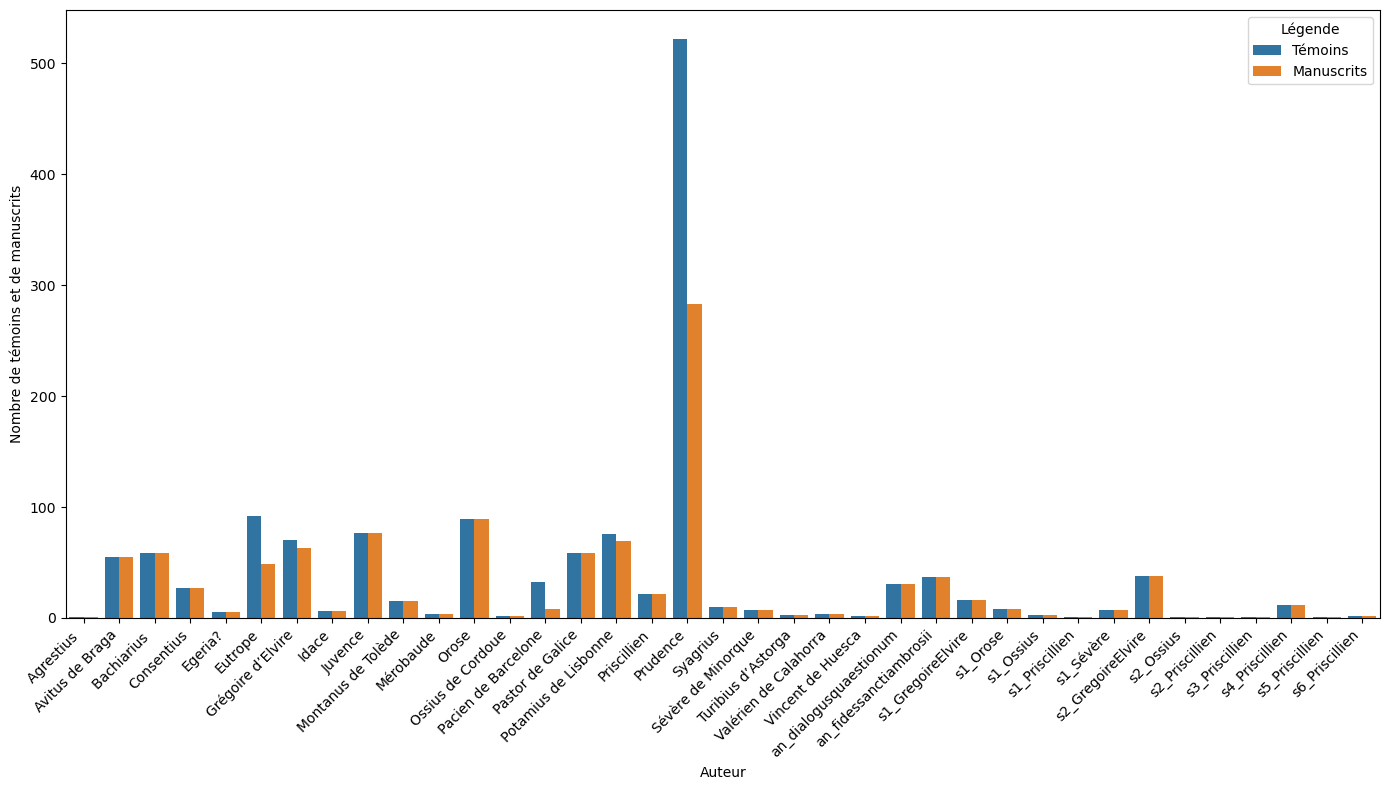
\includegraphics[width=\textwidth]{img/auteursdiff.png}  
	\caption{\textbf{Témoins et manuscrits : répartition par auteur}}
	\label{fig:monimage}
\end{figure}

Nous avons ensuite choisi de limiter ce graphique aux auteurs pour lesquels le nombre de témoins diffère significativement de celui des manuscrits :

\begin{figure}[H]
	\centering
	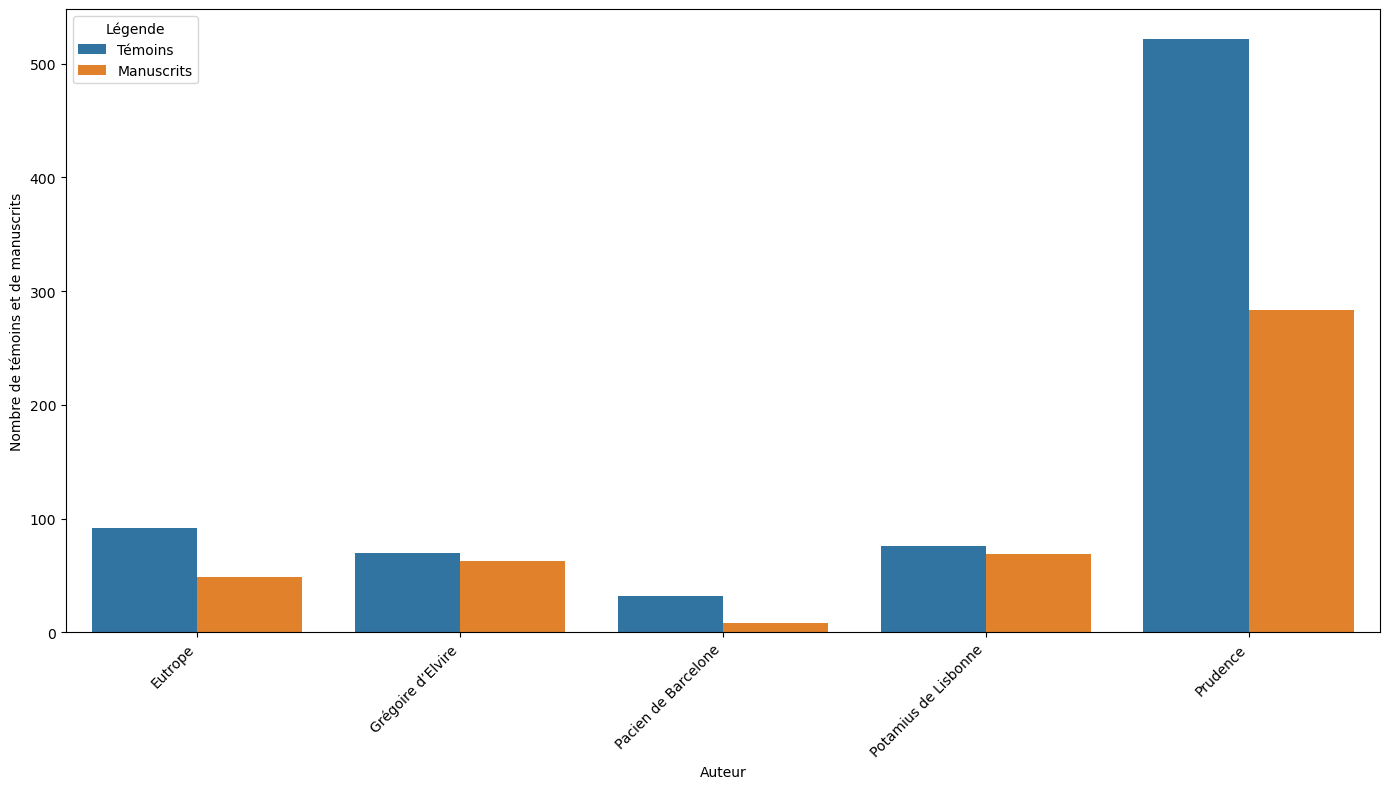
\includegraphics[width=\textwidth]{img/auteursrestriction.png} 
	\caption{\textbf{Représentation graphique en barres des auteurs présentant des différences entre le nombre de manuscrits et de témoins}}
	\label{fig:monimage}
\end{figure}

Pour ces cinq auteurs, cela suggère que plusieurs de leurs textes ont circulé dans un même manuscrit. Est-ce un choix qui a été opéré à un moment
donné par un copiste que de rassembler les textes d’un même auteur? Ou est-ce un choix éditorial de l’auteur que de les transmettre collectivement et non individuellement? Quelles sont les raisons de cette transmission collective?

Du prêtre Eutrope, subsistent trois lettres et un traité. Dans notre ouvrage de référence \textit{Traditio patrum : Scriptores Hispanae}, M.M. Romano qui a rédigé l’article sur Eutrope précise que «\textit{la storia della transmissione del neonato corpus di Eutropio è disorganica; non esiste una vera e propria tradizione comune delle quattro opere, ma esse si diffondono
	separemente [...]}». \footcite[p. 388]{TradPat} Les résultats que nous avons obtenu sur le graphique semble contredire en partie cette affirmation. 92 témoins rapportent ses compositions mais ils sont contenus dans à peine 49 manuscrits. Cela laisse penser que dans la tradition manuscrite de cet auteur, il y a eu une volonté de transmission collective de ses oeuvres. Il faut avant tout préciser que les études qui ont été faites sur Eutrope sont assez réduites, bien qu’elles soient de qualité.  Les principales sont
celles de G. Morin, J. Madoz et P. Courcelle\footcite{Morin, Madoz, Courcelle}
et elles datent toutes du XX\textsuperscript{e} siècle
. D’ailleurs, l’attribution de quatre œuvres à Eutrope est une opinion tardive du même siècle que l’on doit à ces philologues. Bien que les manuscrits contenant les compositions qui lui ont été attribuées aient été recensés, il n’existe pas de véritable étude portant spécifiquement sur les caractéristiques de sa tradition manuscrite et la transmission de ses textes. C’est pourquoi ce qui va être démontré ci-dessus reste au stade d’hypothèses. Tout d’abord, on note un tout cohérent entre les trois lettres : que ce soit l’\textit{Epistula de vera circumcisione} (\textit{CPL}, 566), l’\textit{Epistula de perfecto homine} (\textit{CPL}, 566a), ou l’\textit{Epistula de contemnenda haereditate} (\textit{CPL}, 565), ces lettres font unité puisqu’elles ont toutes été composées dans un même contexte. Elles s’adressent aux mêmes destinataires, autrement dit à deux sœurs qui ont été déshéritées par leurs parents pour s’être vouées à leur foi religieuse. On suppose donc qu’elles forment une correspondance\footnote{On pourrait même dire qu’Eutrope exerce une forme de direction de conscience par correspondance interposée, à l’instar de ce que fit, par exemple, saint Jérôme avec plusieurs grandes dames romaines dans ses \textit{Lettres}.}, transmise telle quelle dans les manuscrits afin de préserver son unité.  Il reste la question du traité \textit{De similitudine carnis pecati} (\textit{CPL}, 567) : en réalité, il s’avère que c’est également une lettre-traité, adressée à \textit{Caesaria}, l’une des deux sœurs déshéritées. La critique met souvent cette lettre-traité à part car sa relation avec les autres n’a été découverte que très tardivement : on doit cette découverte à J. Madoz\footcite{Madoz}. G. Morin a validé cette attribution alors qu’il avait lui-même attribué cette lettre-traité à Pacien de Barcelone\footcite[p. 31--150]{Morin}. Ce ne sont donc pas les trois compositions mais les quatre compositions d’Eutrope qui forment un tout cohérent. Mais l’hypothèse d’une thématique et d’un contexte de composition communs ne suffit à justifier leur
transmission collective. En regardant de manière plus macroscopique le contenu des manuscrits dans lequel elles ont été transmises, on se rend compte qu’elles sont au sein d’un corpus hiéronymien ou pseudo-hiéronymien. A ce sujet, on peut notamment citer le manuscrit Paris, BN, 1688 (\textit{M}) où l’on trouve le premier corpus des lettres d’Eutrope après des lettres authentiques
de Saint-Jérôme.\footcite[p. 379]{Courcelle} Nos propres recherches ont également amené à identifier, entre autres, le manuscrit Vaticano, BAV, 344 qui contient aussi un important corpus hiéronymien et dans lequel est compris les compositions d’Eutrope. D’ailleurs,  les trois lettres \textit{Epistula de vera circumcisione}, \textit{Epistula de perfecto homine}, et \textit{Epistula de contemnenda haereditate} sont les lettres II,  VI et XIX des \textit {Opera supposititia} de Saint-Jérôme  au tome XXX de la  \textit{Patrologia Latina}  éditée par J.-P. Migne \footcite{migneCollection}. Ainsi, le lien des compositions d’Eutrope  avec un « dossier » de textes plus grand, qui se trouve être ici le corpus hiéronymien ou pseudo-hiéronymien explique en partie leur transmission collective. Il faut donc voir au-delà de la transmission individuelle des textes de cet auteur et se placer dans un corpus plus large.

Le cas de Pacien de Barcelone est différent. Des trois textes de cet auteur, 32 témoins sont parvenus jusqu’à nous, contenus dans seulement 8 manuscrits. Cette répartition indique que pour la plupart des cas, l'ensemble des textes ont été transmis dans un même manuscrit. C. Granado, C. Épitalon et M. Lestienne dans leur édition critique de Pacien de Barcelone \footcite{Granado} n'ont pas évoqué cet aspect de la transmission des textes de cet évêque. S.I. Abellán et J.C. Martín Iglesias dans \textit{Traditio Patrum, Scriptores Hispanae} ne donne pas plus d’indications à ce sujet. Tout ce que l’on peut dire sur de cette transmission collective des textes est qu’elle est attestée très précocement dans la tradition manuscrite. En effet, en se penchant sur le \textit{stemma} des œuvres de Pacien de Barcelone \footcite [p. 366]{TradPat}, on se rend compte que non seulement les textes sont regroupés en un seul \textit{stemma} mais en plus toute la tradition manuscrite découle d’un unique manuscrit, le Vaticano, BAV, Reg. Lat. 331(\textit{R}), datant du IX\textsuperscript{e} siècle. Il contient l’oeuvre complète de Pacien, des feuillets 39r à 76r.  Il est donc vraisemblable que l'archétype ait été un volume comprenant les oeuvres complètes de cet auteur. Si l’on se penche plus réticulairement sur les trois compositions de Pacien, on se rend compte qu’elles traitent toutes de la même thématique : chacun de ces opuscules et chacune de ces lettres abordent sous une forme différente, le problème de la pénitence, sujet fort débattu dans l'Église primitive, et notamment la question de savoir si le pardon des péchés commis après le baptême est ou non légitime. Pacien affirme également sa position contre les novatiens, qui refuse quant à eux toute pénitence post-baptismale. On peut donc émettre l’hypothèse que la transmission des textes de Pacien s’est faite collectivement car ces derniers représentent un corpus unitaire doctrinal : l’ensemble de son œuvre est anti-novatienne. 

Pour Prudence, la question d'une oeuvre unitaire n'est plus à démontrer. L'ensemble de son oeuvre est  pourvu d'une unité organique, puisque l'ordre des poèmes les uns par rapport aux autres a été voulu par l'auteur et témoigne d'une organisation stylisée. Avant tout, la forme métrique des quatre textes principales du recueil de Prudence permet de les ramener à l'unité : on a deux oeuvres lyriques (\textit{Cathemerinon} et \textit{Peristephanon}) encadrant quatre oeuvres dactyliques à finalité globalement didactique (\textit{Liber Apotheosis, Hamartigenia, Psychomachia, Contra Symmachum}). Mais ce qui interpelle dans l’œuvre de Prudence, ce sont deux compositions nommées \textit{Praefatio} et \textit{Epilogus}. La question à se poser est donc : ces deux compositions sont préliminaires et conclusives de quelle oeuvre ? La critique de Prudence a largement débattu dessus et les réponses qui y ont été portées sont loin d’être admises à l’unanimité.  J.-L. Charlet dans son article « La poésie de Prudence dans l'esthétique de son temps », affirme qu’il « s’agit non d’une préface au seul recueil du \textit{Cathemerinon}, mais d’une préface générale, à laquelle répond à la fin l’\textit{Epilogus}.» \footcite{Charlet}. Pour lui, « les différents poèmes de Prudence ne sont donc pas des œuvres indépendantes ou isolées : ils constituent un tout cohérent, tant sur le plan poétique que sur le plan spirituel […] » \footcite[p. 369]{Charlet} . Dans sa thèse, W. Ludwig emploie même le terme de « super-poème~» pour qualifier l’œuvre de Prudence \footcite{ludwig1977}. D’autant plus qu’ I. Lana dans son étude sur Prudence avance que cet évêque aurait composé ses poèmes en même temps, sans grand écart chronologique (entre 398 et 404 plus précisément)\footcite[24]{Lana}. On voit donc une volonté d’unité jusque dans la genèse de ses poèmes. Au regard de ce qui a été dit, il semble logique que les compositions de Prudence aient été transmises collectivement. Les transmettre individuellement reviendrait pour un copiste à ne  copier qu’un fragment de ce « super-poème ».  J.-L. Charlet précise même que c’est « Prudence qui a voulu représenter ses poèmes dans un certain ordre et que cette volonté a été suivie par une bonne partie de la tradition manuscrite, qu’elle remonte au poète lui-même ou à celui qui se serait chargé de l’éditer après sa mort » \footcite[p. 370]{Charlet}.  Ainsi, on voit que dans le cas de Prudence, la transmission collective est due à une volonté éditoriale de l’auteur lui-même.

Le cas de Grégoire d'Elvire est beaucoup plus épineux. Pour cet auteur, nous avons mis en place une fonction permettant d’identifier précisément les textes qui ont été transmis au sein d’un même manuscrit. Il en ressort que la différence entre le nombre de manuscrits et de témoins s’explique notamment par le fait que nous avons considéré les livres 1 et 2, d’une part, et les livres 3 et 5 du \textit{Tractatus V de Epithalamio}, d’autre part, comme deux textes distincts dans notre jeu de données. Si cela constitue une entorse à l’unité organique du texte, ce choix s’est imposé dans la mesure où E. Schulz-Flügel dans son édition critique a jugé bon de produire un \textit{stemma codicum} pour chacun de ces ensembles. Pour ce critique, les livres 1-2 et 3-5 doivent être envisagés séparément à cause de leur tradition manuscrite. Les livres 1 et 2 ont fait l'objet d'une révision de la part de leur auteur (notamment par une transformation du commentaire en une forme à caractère homilétique) et il est très probable que ce dernier n'ait pas eu le temps de l'étendre aux trois derniers livres.  Dès lors, cette seconde version des livres 1 et 2 a connu une circulation indépendante, intégrée par E. Schulz-Flügel dans un \textit{stemma codicum} propre aux deux premiers livres. Puisque notre étude porte sur la dynamique de transmission des textes, nous avons choisi de considérer séparément les livres composant ce même texte. Dans une démarche philologique, il est probable que nous aurions préféré conserver l’œuvre dans son unité globale, mais l’approche adoptée ici requiert cette distinction.


Le dernier de nos auteurs pour lequel le nombre de témoins diffère de celui des manuscrits est Potamius de Lisbonne. En utilisant la même fonction que pour Grégoire d'Elvire, on constate que deux homélies, \textit{De Lazaro} (\textit{CPL}, 541) et \textit{De martyrio Esaiae prophetae} (\textit{CPL}, 543) ont, au moins en partie, connu une transmission commune. M. Conti, dans la section qu’il consacre à Potamius de Lisbonne dans le volume \textit{Corpus Christianorum : Tradition Patrum}, souligne que cette co-transmission résulte d’une attribution erronée des deux textes à Zénon de Vérone\footcite[p. 43 et 54]{TradPat}. Cette erreur avait déjà été relevée par deux critiques italiens, P. et G. Ballerini, qui, en publiant une nouvelle édition critique des homélies de Zénon de Vérone, ont signalé plusieurs homélies apocryphes, parmi lesquelles figuraient nos deux textes, le \textit{De Lazaro} et le \textit{De martyrio Esaiae prophetae}. Ce sont d’ailleurs ces deux frères qui ont proposé de les attribuer à l’évêque Potamius\footcite[p.~ XXX--XXXI]{Ballerini}, attribution reprise ensuite par les critiques Andrea Galland\footcite[p. 96--99]{Galland} et Jacques-Paul Migne\footcite[coll. 1411--1415]{migne8}. \\

\begin{center}
	\textit{Conclusion partielle}
\end{center}

La comparaison entre le nombre de témoins et de manuscrits  révèle des schémas intéressants chez certains auteurs. Grégoire d'Elvire, Prudence, Eutrope,  Pacien de Barcelone et Potamius se distinguent par un nombre de témoins  supérieur au nombre de manuscrits. Pour Prudence, cette distribution suggère une transmission collective de ses textes, probablement due à une volonté éditoriale de l'auteur. Chez Eutrope, Potamius et Pacien, bien que la documentation soit moins abondante, la concentration des témoins dans un nombre restreint de manuscrits suggère elle aussi une transmission collective. Pour les deux premiers, celle-ci s’explique par l’intégration de leurs œuvres dans un corpus plus vaste (respectivement celui de saint Jérôme et de Zénon de Vérone), sans conteste liée à une attribution erronée de l’auteur. Pour l'autre, l'anti-~novationisme qui infuse l'ensemble de ses textes en est sûrement la raison puisque cette prise de position constante représente une unité thématique et doctrinale. Le cas de Grégoire d'Elvire est à part : bien que ces livres forment une seule et même oeuvre, nous considérons les livres 1-2 et 3-5 comme deux textes différents en raison de leur transmission textuelle indépendante due à une révision des deux premiers livres.

Ce phénomène de co-transmission que nous observons est typique pour les textes de l'Antiquité tardive : comme le souligne S. Gioanni dans \textit{L'Antiquité tardive dans les collections médiévales}, « les textes de l'Antiquité tardive ont été pour la plupart transmis par des collections médiévales ». Leurs modes de constitution étaient très différents et dépendaient en partie des acteurs médiévaux : S. Gioanni et B. Grévin précisent dans leur introduction que les mises en recueil pouvaient être auctoriales, génériques, mais aussi thématiques. Cela peut expliquer, de fait, la mise en corpus des textes de Pacien au cours de leur transmission puisqu'elles représentaient une unité doctrinale. Un autre cas de transmission doctrinale est Turibius d'Astorga dont le texte \textit{Epistula ad Idacium et Ceponium} (\textit{CPL}, 564) a été transmis dans un corpus anti-priscillaniste. Il est également important de souligner que « d'autres recueils ont été réalisés dans l'Antiquité tardive par des collectionneurs soucieux de transmettre des œuvres qu'ils jugeaient importantes [...] auxquels ont largement puisé les collections médiévales»\footcite[p.5]{collectionAT}. On peut donc aisément supposer que la mise en recueil des textes d'Eutrope avec les œuvres hiéronymiennes ou pseudo-hiéronymiennes était due à cette pratique. Eutrope n’appartient pas au corpus hiéronymien, mais c’est cette association fautive qui a favorisé sa diffusion. Il n'est d'ailleurs pas le seul de notre corpus, Sygrius a aussi été transmis dans un corpus hiéronymien. Une autre pratique était la mise en recueil générique : les collections liturgiques comme les homéliaires ou les recueils de sermons étaient très répandues au Moyen-Âge. Notre corpus était composé en partie d'homélies et de sermons, on peut supposer que certaines ont été transmises grâce à cette mise en recueil. 


Suite à ces considérations, se pose la question du degré de granularité que nous accorderons à ses textes, leurs témoins  ainsi que les manuscrits qui les transmettent. En effet, dans un contexte où des recueils peuvent avoir été conçus unitairement par les auteurs, ou bien dépendre de la tradition, quel est le niveau d'oeuvre que nous allons rendre applicable aux textes? Même si notre corpus est exhaustif pour la période et la zone géographique concernées, il demeure quantitativement petit pour les analyses à venir.  C'est pourquoi nous avons décidé que seuls les textes de Prudence seraient réunis en un  corpus prudencien. Il s’agit en effet du seul auteur dont la mise en recueil des textes ne procède pas d’un processus de transmission postérieur, mais bien d’une volonté autoriale initiale attestée. Les textes des quatre autres auteurs ne seront pas unifiés sous une seule œuvre  et ils seront de fait considérés comme indépendants les uns des autres.

\section{Premières analyses exploratoires du corpus}

\subsection{Distribution des données}
Nous souhaitons effectuer une première analyse exploratoire de notre corpus en nous intéressant à la répartition des données. Il va de soi que des variables telles que le nombre de manuscrits ou de témoins par texte ne suivent pas une loi normale gaussienne. C'est pourquoi l'objectif est de voir si nos données s'intègrent bien à une autre loi. Nous présupposons une loi à queue lourde puisque cela est très fréquent dans les phénomènes sociaux.

Après avoir regroupé les textes selon leur nombre de témoins, un graphique en échelle logarithmique a été tracé afin de visualiser la distribution :

\begin{figure}[H]
	\centering
	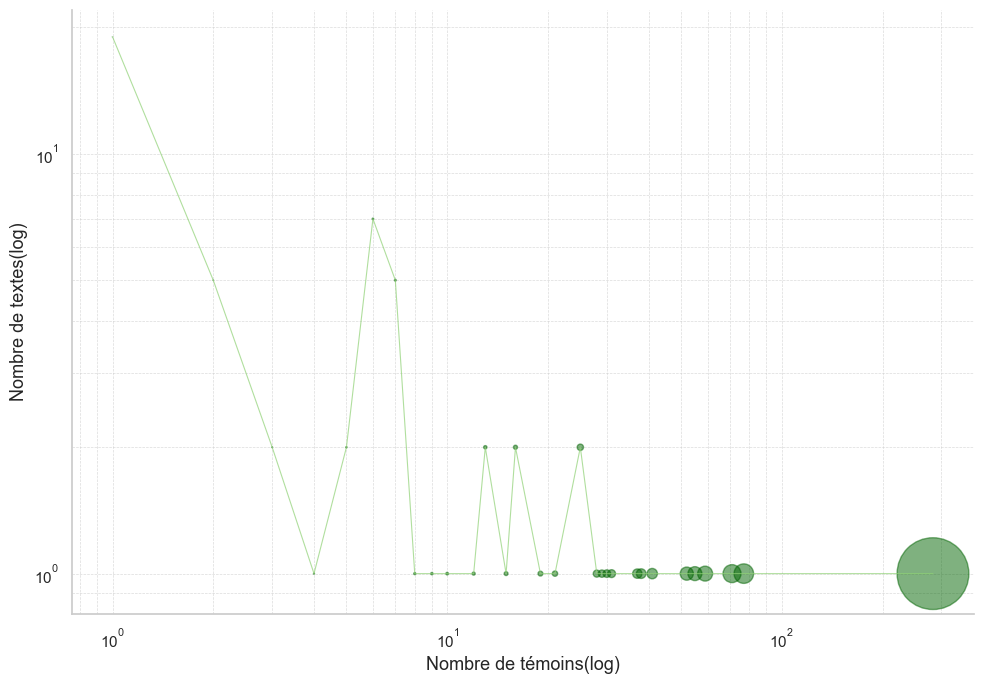
\includegraphics[width=\textwidth]{img/logtextetemoin.png} 
	\caption{\textbf{Distribution des textes selon le nombre de témoins (échelle log-log)}} 
     La taille des points est proportionnelle au nombre de témoins.
	\label{fig:monimage}
\end{figure}

On constate que notre distribution est très déséquilibrée : une importante partie des textes ont seulement 1 témoin tandis qu'une minorité de textes présentent quant à eux un nombre assez élevé de témoins. Cela signifie que les textes largement diffusés sont peu fréquents dans notre corpus mais significatifs. Ce type de distribution est typique pour une loi de distribution à queue lourde.
Afin d’être encore plus précis, nous allons tenter d’identifier à quelle loi à queue lourde notre distribution s’ajuste le mieux. Bien entendu, nous avons conscience de la taille réduite de notre corpus et, par conséquent, nous ne nous attendons pas à un ajustement parfaitement fidèle à une loi théorique. Cette exploration reste néanmoins intéressante à mener.\\
Pour se faire, nous avons utilisé la librairie \texttt{powerlaw} de Python, qui permet entre autres de faire des analyses de distribution sur des lois à queue lourde. Un point est néanmoins à souligner : nous ne pouvons pas fournir à cette librairie notre comptage de fréquences comme cela a été fait dans le graphique précédent où les textes ayant le même nombre de témoins étaient regroupés. En effet, \texttt{powerlaw} ne prend en entrée que des observations individuelles, c’est-à-dire le nombre de témoins associé à chaque texte.
Il suffit ensuite d’utiliser la fonction \texttt{powerlaw.Fit} qui ajuste une loi de puissance à nos données. Cette dernière permet également d’afficher l’exposant \(\alpha\), ce qui donne une indication sur la pertinence de l’ajustement à une loi de puissance. Dans notre cas, \(\alpha = 1{,}407\) : nous avons affaire à une loi lourde en queue, puisque \(\alpha \in [1,2]\). Toutefois, cet indicateur n'appartient pas à la plage typique \([2,3]\), souvent considérée comme un critère mathématique pour confirmer la présence d’une véritable loi de puissance. C'est pourquoi la comparaison avec d'autres lois de distribution à queue lourde s'annonce nécessaire. Une fonction est déjà prévue à cet effet dans \texttt{powerlaw} : grâce à \texttt{fit.distribution\_compare}, nous pouvons comparer l’ajustement de nos données à une loi de puissance, en le confrontant à celui de deux autres distributions de référence, l’exponentielle et la log-normale.

\begin{figure}[H]
	\centering
	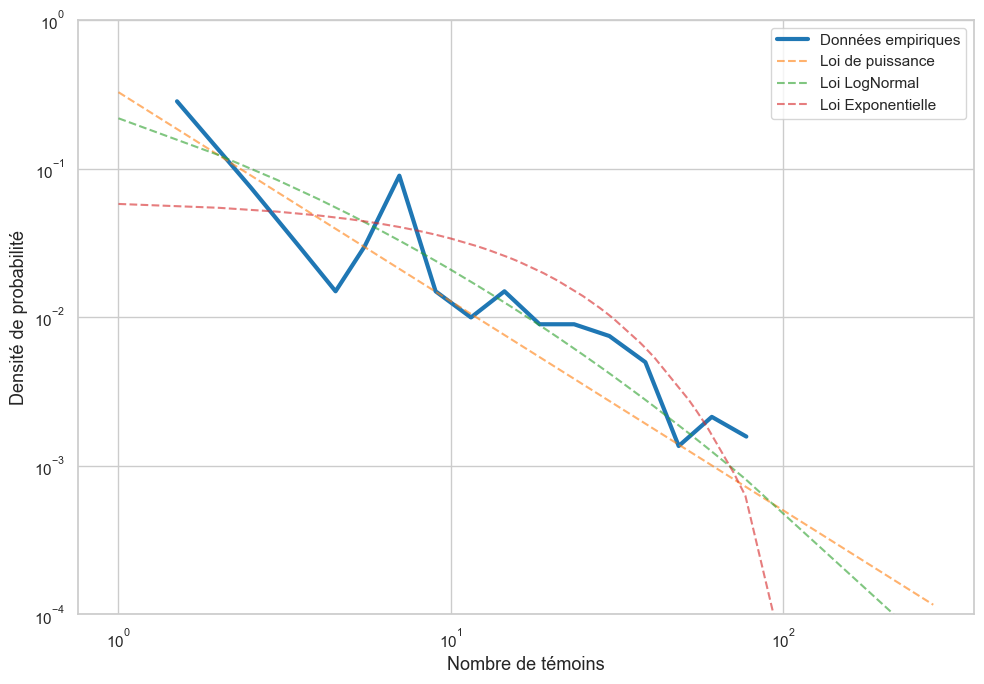
\includegraphics[width=\textwidth]{img/comparelaw.png} 
	\caption{\textbf{Ajustement de la distribution du nombre de témoins par texte à différentes lois : puissance, lognormale et exponentielle.}}. 
	\label{fig:monimage}
\end{figure}

La lecture du graphique est complétée par un test de vraisemblance, qui permet, à partir du rapport de vraisemblance \(R\) et de la valeur \(p\), de déterminer quelle loi fournit l’ajustement le plus significatif à nos données.

\begin{table}[h!]
	\centering
	\begin{tabular}{lcc}
		\hline
		Comparaison & \(R\) & \(p\)-value \\
		\hline
		Power law vs Lognormal & -8.251 & 0.008 \\
		Power law vs Exponential & 14.710 & 0.303 \\
		\hline
	\end{tabular}
	\caption{\textbf{Résultats du test de comparaison des ajustements entre la loi de puissance et d’autres lois.}}
	\label{tab:distribution_compare}
\end{table}

Pour le test de comparaison entre la loi de puissance et la loi lognormale, on constate que \(R\) est négatif, ce qui indique que la loi lognormale s’ajuste mieux à nos données. De plus, la valeur \(p\) est inférieure à 0,05 ce qui signifie que cette différence est statistiquement significative. À l’inverse, pour le test entre la loi de puissance et la loi exponentielle, bien que \(R\) soit positif, suggérant que la loi de puissance est préférable, la valeur \(p\) est supérieure au seuil de 0,05. On ne peut donc pas affirmer avec certitude que la loi de puissance est préférable à la loi exponentielle sur nos données. \\

%Au regard de la courbe, on constate que nos données empiriques forment une courbe non-lisse, sujette à une forte variabilité locale, ce qui rend l’ajustement visuel aux trois lois de distribution (loi de puissance, lognormale et exponentielle) difficile. Ce graphique nous signale ainsi que notre échantillon est restreint, et qu’il faut donc rester précautionneux dans nos conclusions concernant l’ajustement des lois.

En définitive, notre analyse exploratoire révèle que la distribution du nombre de témoins par texte s’apparente à une loi à queue lourde et les résultats obtenus suggèrent que la loi lognormale offre un ajustement statistiquement plus pertinent que la loi de puissance proprement dite. Ce constat, confirmé par les tests de vraisemblance, invite donc à nuancer l’hypothèse initiale d’un véritable modèle en loi de puissance, du moins dans l’état actuel de notre corpus. Il faut préciser que la structure même de ce dernier, caractérisé par une forte concentration de textes faiblement transmis et par quelques textes largement diffusées, reflète des réalités historiques de la circulation textuelle qui ne se prêtent pas aisément à des distributions purement théoriques. De plus, la taille limitée de notre échantillon peut également expliquer cette distribution hétérogène, empêchant peut-être la manifestation claire d’une loi de puissance. 

\subsection{Aperçu philologique et computationnel des \textit{stemmata codicum} de notre corpus}
\label{stemmata}

Comme indiqué dans la partie \ref{Critères de sélection du corpus}, lors de la collecte des données, nous avons également relevé le \textit{stemma codicum} associé à chaque texte, lorsque celui-ci était disponible. Il semble donc pertinent d’examiner si ces \textit{stemmata} présentent certaines similarités stemmatiques, comme la bifidité, l’équilibre ou non des branches, ou encore les types de témoins pris en compte.

\subsubsection{Présentation et ajustements des \textit{stemmata codicum}}
	
L'ensemble des \textit{stemmata} que nous avons récolté pour les textes des Pères de l'Eglise en péninsule Ibérique ont été versés dans la base \textit{OpenStemmata}, comme cela a déjà été précisé. Une précision s’impose néanmoins~: les \textit{stemmata} versés sont reproduits dans leur forme exacte, telle qu’elle apparaît dans les différentes éditions critiques. Dans le cadre de notre étude, nous rappelons que nous ne prenons en considération que les témoins relevant de la tradition directe, et uniquement dans la mesure où ces témoins sont transmis par l’objet matériel qu’est le manuscrit, et ce, jusqu’au XV\textsuperscript{e} siècle inclus.
Cela étant dit, certains \textit{stemmata} ont dû faire l’objet de modifications afin de répondre à nos critères de sélection. Ces ajustements sont au nombre de trois~:
	
	\begin{itemize}
		\item la suppression de témoins lorsque ceux-ci dépendent d’éditions, ou sont eux-mêmes des éditions~;
		\item l’élimination des témoins relevant de la tradition indirecte~;
		\item l’exclusion des manuscrits dont la datation est postérieure au XV\textsuperscript{e} siècle. \\
	\end{itemize}
	
	Plus précisément, voici un aperçu des \textit{stemmata} qui ont été modifiés:
	
	\begin{itemize}
		
		\item Pacien de Barcelone (\textit{CPL} 561, 562 et 563) : suppression de la branche avec les témoins descendants de la \textit{Collectio ex dictis XIII patrum} de Floro de Lyon.\footnote{Cette collection se présente comme un commentaire des épîtres de Saint Paul, rédigé à partir de citations de douze Pères de l'Église, dont notamment Pacien de Barcelone. Elle a été éditée récemment (2002--2007) dans le \textit{Corpus Christianorum, série Continuatio Medievalis} (193, 193 et 193B). Pour les passages sur Pacien de Barcelone, voir p.~VII--XIII et p.~1--27 (\textit{CC CM}, 193B).} On supprime également la branche contenant les témoins issus de l’\textit{editio princeps} réalisée par J.~Du Tillet.\footcite{Dutillet}
		
		
		\item Idace (\textit{CPL}, 2263) : suppression des témoins postérieurs au~XV\textsuperscript{e}~siècle ainsi que des témoins de la tradition indirecte, c’est-à-dire des textes comprenant pour la plupart des épitomés de sa \textit{Chronique} : le témoin \textit{IP} (qui représente le texte d’Isidore de Séville, \textit{Historia Gothorum, Wandalorum et Suevorum}, \textit{CPL}~1204), le témoin \textit{F} ainsi que ceux qui en dérivent (représentant le \textit{Frédégaire}, qui compile à la fois Idace et Isidore), le témoin \textit{G} (texte de la \textit{Chronica Gallica ad annum DXI}, \textit{CPL}~2259), le témoin \textit{M} (correspondant au \textit{Chronicon Luxoviense}), ainsi que les témoins \textit{T} et \textit{S} (représentant respectivement la \textit{Chronographia} de Sigebert de Gembloux et le \textit{Chronicon abbatiae Palidensis}).
		
		\item Syagrius (\textit{CPL}, 560) : suppression de deux témoins postérieurs au XV\textsuperscript{e}~siècle (\textit{S} et \textit{O}).
		
		\item Montanus de Tolède  (\textit{CPL}, 1094) : suppression de trois témoins postérieurs au XV\textsuperscript{e}~siècle (\textit{Ma}, \textit{Vat} et \textit{Bal}). %Nous attirons l'attention sur le fait que les deux lettres de Montanus font partie de la Collection Canonique d'Espagne et de fait le \textit{stemma} entier dépend de la \textit{recensio Vulgata}. A COMPLETER
		
		
		
		
	\end{itemize}
	
	
	
Certains des \textit{stemmata} récoltés seront quant à eux écartés, car leurs nœuds ne correspondent pas à des témoins individuels mais à des collections ou à des familles de manuscrits, ce qui s’avère trop imprécis pour nos analyses. C’est le cas du texte de Pastor de Galice : son symbole de foi, le \textit{Libellus in modum symboli} (\textit{CPL},~559), composé à l’occasion du premier concile de Tolède, doit sa survie à sa circulation dans diverses collections canoniques.\footcite[Pour une vue chronologique et systématique des collections canoniques, voir][]{kery, Hispana}
 Il apparaît notamment dans les collections \textit{Hispana}, \textit{Hispana Gallica}, \textit{Hispana Gallica Augustodunensis}, \textit{Pseudoisidoriana}, \textit{Hadriano-Hispanica}, \textit{Sancti-Amandi}. Le \textit{stemma} proposé par S.~Iranzo-Abellán et J.~C.~Martín-Iglesias dans \textit{Traditio Patrum}\footcite[p. 349]{TradPat} représente dès lors une généalogie de ces différentes collections canoniques à travers lesquelles ce symbole de foi a été transmis, plutôt qu’un \textit{stemma} des témoins eux-mêmes.
	Un autre \textit{stemma} qui a été écarté de nos analyses est celui qui a été réalisé pour l'\textit{Epistula ad Palchonium}  (\textit{CPL},~575) d'Avitus de Braga puisque les nœuds sont  des familles de manuscrits \footnote{Les familles de manuscrits ont été établies par E. Vanderliden dans son édition critique «Revelatio Sancti Stephani», \textit{Revue des études byzantines}, 4 (1946), p. 178-217.}. Il en va de même pour le \textit{Fides « ~Sancti Ambrosii~ »}  (\textit{CPL},~789) dont la tradition manuscrite est divisée en cinq familles de manuscrits correspondant à des collections canoniques et un manuscrit indépendant \footcite [p. 237-242]{TradPat}. 
	
\subsubsection{Analyse computationnelle des propriétés stemmatiques}

Avant de nous lancer dans notre analyse computationnelle, quelques éclaircissements sur la méthode stemmatique s'impose. L’une des méthodes les plus répandues pour construire un \textit{stemma codicum} est la méthode lachmannienne, fondée sur l’identification des « fautes communes »\footnote{Nous tenons à préciser que K. Lachmann est à l'origine de la méthode de reconstruction généalogique des textes, mais c'est le philologue P. Lejay qui en 1903, lors de la publication de l'édition critique des \textit{Oeuvres} d'Horace, va formuler de manière explicite ce qui restait jusque-là quelque peu implicite : ce sont les innovations communes, autrement dit les fautes partagées, qui sont les plus probantes.}. Elle repose sur le principe selon lequel une communauté d’erreurs implique une unité d’origine. En d’autres termes, on tente de reconstituer l’histoire d'un texte à partir des relations entre ses témoins, en partant du postulat que tous dérivent d’un ancêtre commun, l’archétype, et qu’ils se répartissent en branches ou familles selon leurs fautes propres ou partagées.
La construction d’un tel \textit{stemma} repose sur plusieurs étapes successives et méthodiques. On commence par la \textit{recensio codicum}, c’est-à-dire l’inventaire systématique des témoins manuscrits, qu’ils appartiennent à la tradition directe ou indirecte, sans oublier les éditions antérieures.
Suit ensuite la \textit{collatio}, qui consiste à comparer les textes transmis par les différents manuscrits afin d’identifier  les leçons divergentes. Cette phase est primordiale, car elle fournit les données qui permettront de déterminer les relations entre les témoins.
À partir de cette comparaison s’engage la \textit{selectio codicum} : il s’agit de choisir les manuscrits à retenir pour l’établissement du texte critique. Certains témoins sont écartés à ce stade, notamment ceux qui sont trop contaminés ou ceux qui ne sont que des copies fidèles de manuscrits mieux conservés.
Enfin, on procède à l’\textit{ordinatio codicum}, autrement dit au classement des témoins. Cette étape consiste à regrouper les manuscrits en classes, sous-classes, familles ou branches généalogiques, selon les erreurs partagées, mais aussi en tenant compte d’éléments codicologiques ou paléographiques. C’est à l’issue de ce processus qu’on peut établir le \textit{stemma codicum}, qui visualise les relations de filiation entre les témoins, de l’archétype originel jusqu’aux copies les plus tardives.

Cette méthodologie de reconstitution de l’histoire d’un texte, bien que rigoureuse dans ses principes, a néanmoins été interrogée quant aux biais qu’elle peut induire chez ceux qui la mettent en œuvre. À cet égard, le débat lancé par le philologue français J. Bédier autour de la bifidité des \textit{stemmata} constitue un exemple emblématique des limites potentielles d’une approche qui se voulait pourtant objective.
 En effet, en 1928, J. Bédier  remarquait que la plupart des \textit{stemmata} élaborés par ses contemporains adoptaient une structure étonnamment récurrente : la racine de l’arbre, censée représenter l’archétype, ne donne presque toujours naissance qu’à deux branches directes. Cette bifurcation systématique (que Bédier observe dans plus de 95\,\% des cas) lui apparaît comme la conséquence d’un biais inconscient lié à la manière dont les philologues mettent en œuvre la méthode lachmannienne. Il s’agirait donc, selon lui, d’un défaut structurel de la méthode elle-même. Ce constat a donné lieu à une controverse méthodologique de fond, encore vive aujourd’hui, opposant deux écoles : d’un côté, les partisans de la méthode de Lachmann, attachés à ses principes classificatoires stricts et de l’autre, les héritiers de Bédier, qui privilégient une approche plus historique fondée sur l’autorité présumée des meilleurs manuscrits, souvent édités sans recours à un \textit{stemma}.  
 D’autres traits récurrents des \textit{stemmata} peuvent d’ailleurs être relevés, comme la tendance à l’asymétrie : certains arbres présentent des branches nettement moins fournies, reflet probable de processus d’extinction survenus au cours de la transmission textuelle.
 
À l’heure de l’informatique et de l’essor des méthodes computationnelles, il devient aisé de quantifier ces propriétés stemmatiques afin de voir si certaines tendances s'en dégagent. Certes, en ayant éliminé certains de nos \textit{stemmata}, nous avons pleinement conscience que l’analyse ne portera que sur une fraction réduite de la tradition étudiée ; néanmoins, cela peut offrir un premier aperçu instructif. Le dépôt GitHub \texttt{ExtinctionOfTexts}\footcite{extinction_texts_github} du projet \textit{LostMA} met à disposition un code permettant justement de quantifier certaines caractéristiques structurelles des arbres stemmatiques. Conçu à l’origine pour comparer des simulations d’arbres générés par un processus de naissance et de mort à des données empiriques, ce code offre une base intéressante pour nos propres analyses. Nous l’utilisons ici afin d’examiner certaines propriétés stemmatiques présentes dans nos arbres empiriques:
\begin{itemize}
	\item la proportion de nœuds internes de degré 2 ou 3,
	\item la fréquence des arbres dont la racine est bifide,
	\item la proportion d’arêtes reliant des témoins vivants,
	\item un indice d’asymétrie des arbres.\\
\end{itemize}


Le code calcule ces différentes propriétés stemmatiques en s'appuyant sur une procédure statistique de \textit{bootstrap}. En quelques mots, il s'agit de générer un grand nombre d’échantillons aléatoires avec remise, à partir des arbres disponibles, afin d’estimer non seulement la valeur moyenne de chaque mesure, mais aussi un intervalle de confiance autour de cette estimation. Dans notre cas, l’intervalle de confiance est fixé à 10 \%. Avant toute estimation, les \textit{stemmata} subissent un pré-traitement: ils sont nettoyés en supprimant par exemple les nœuds isolés. Les cas de contamination (nœuds à plusieurs parents) sont réduits à une seule filiation (choisie aléatoirement) pour obtenir un arbre simplifié. Enfin, les témoins attestés sont distingués des nœuds hypothétiques.

\begin{table}[H]
	\centering
	\begin{tabular}{lccc}
		\toprule
		\textbf{Observable} & \textbf{Valeur estimée} & \textbf{Borne inférieure} & \textbf{Borne supérieure} \\
		\midrule
		Proportion de \textit{stemmata} bifides          & 0{,}67 & 0{,}33 & 0{,}92 \\
		Déséquilibre i3                                     & 0{,}13 & 0{,}03 & 0{,}29 \\
		Proportion de nœuds internes de degré 2          & 0{,}08 & 0{,}03 & 0{,}22 \\
		Proportion de nœuds internes de degré 3          & 0{,}02 & 0{,}00 & 0{,}06 \\
		Proportion de témoins descendants directs        & 0{,}12 & 0{,}03 & 0{,}38 \\
		\bottomrule
	\end{tabular}
	\caption{\textbf{Mesures des propriétés stemmatiques avec intervalles de confiance à 10\,\% sur les arbres modifiés.}}
	\label{tab:stemmatic_metrics}
\end{table}

La proportion estimée de \textit{stemmata} bifides atteint 67\,\%, ce qui signifie qu’environ deux tiers des arbres présentent une bifurcation à la racine : ce  résultat est conforme à l’idée de J.~Bédier d’une structure initiale relativement simple, divisée en deux branches. Toutefois, l’intervalle de confiance assez large [0{,}33 ; 0{,}92] indique une forte incertitude, principalement liée à la taille réduite de notre échantillon (\( n = 12 \)). L’observation empirique de certains arbres permet par ailleurs de nuancer ce constat : dans le cas des \textit{Chroniques} d’Idace (\textit{CPL}, 2263), l’absence de bifidité s’explique par la présence de l’autographe à la racine du \textit{stemma}, qui donne ensuite naissance à un archétype $\alpha$, lui-même à l’origine d'un hyperarchétype, $\beta$. Pour Grégoire d’Elvire et son texte \textit{Tractatus V de epithalamio} (\textit{CPL}, 547), le \textit{stemma} repose sur deux archétypes distincts, $\omega_1$ et $\omega_2$ : le premier pour la version initiale des livres I et II du \textit{Tractatus V de epithalamio}, et le second pour la révision de ces mêmes livres opérée par l’auteur lui-même. Ces deux branches mènent ensuite chacune à un hyperarchétype, ce qui donne au final une racine bifide propre à chaque archétype, si on les considère séparément\footnote{Se référer à \ref{stemmabifid}}.
L’indice de déséquilibre $i_3$ est évalué à 0{,}13, ce qui indique que les arbres présentent une structure globalement équilibrée. La proportion de nœuds internes de degré 2 et 3 est très faible (respectivement 0{,}08 et 0{,}02), ce que l’on peut attribuer au fait que certaines branches ou témoins ont été retirés lorsqu’ils étaient jugés trop tardifs ou qu’il s’agissait d’éditions. Par ailleurs, la proportion de témoins reliés directement entre eux (témoins attestés) s’élève à 0{,}12 : environ 12\,\% des liens sont donc établis entre témoins vivants. Toutefois, l’intervalle de confiance [0{,}03 ; 0{,}38] reste large.
En somme, ces résultats offrent un premier aperçu de certaines propriétés structurelles des arbres de notre corpus, mais ils doivent être interprétés avec prudence : les intervalles d’incertitude demeurent élevés en raison de la taille modeste de l’échantillon.

Nous avons alors décidé de mener cette analyse sur les \textit{stemmata} dans l’état où ils apparaissent dans les éditions critiques, c’est-à-dire sans appliquer les modifications que nous avions opérées pour les rendre conformes aux critères de sélection de notre corpus. Autrement dit,nous avons conservé les manuscrits postérieurs au~XV\textsuperscript{e}~siècle, les éditions ainsi que certains témoins issus de la tradition indirecte mais jugés suffisamment significatifs par les critiques pour être intégrés dans le \textit{stemma}. On pense encore une fois au cas d’Idace et de ses \textit{Chroniques}, dont une grande partie des témoins sont en réalité des chroniques d’autres auteurs qui, dans une chaîne successive de réécriture, ont repris des extraits du texte de ce dernier. L’objectif est ici de vérifier si les résultats obtenus varient lorsque l’on travaille sur une version plus « étendue » des arbres.

\begin{table}[H]
	\centering
	\begin{tabular}{lccc}
		\toprule
		\textbf{Observable} & \textbf{Valeur estimée} & \textbf{Borne inférieure} & \textbf{Borne supérieure} \\
		\midrule
		Proportion de stemmata bifides              & 0.74 & 0.42 & 1    \\
		Déséquilibre I3                             & 0.16 & 0.02 & 0.36 \\
		Proportion de nœuds internes de degré 2     & 0.08 & 0.04 & 0.21 \\
		Proportion de nœuds internes de degré 3     & 0.02 & 0    & 0.08 \\
		Proportion de témoins directs descendats     & 0.22 & 0.05 & 0.57 \\
		\bottomrule
	\end{tabular}
	\caption{\textbf{Mesures des propriétés stemmatiques avec intervalles de confiance à 10\,\% sur les arbres non modifiés}}
	\label{tab:observables}
\end{table}

On observe que la proportion de \textit{stemmata} ayant une racine bifide passe de 0{,}67 à 0{,}74. Ce résultat n’a rien de surprenant~: dans certains cas, la racine bifide réapparaît dès lors que l’on conserve certains témoins exclus précédemment. C’est notamment le cas pour les textes de Pacien de Barcelone (\textit{CPL}, 561-563), où l’archétype donne naissance à deux branches~: un hyperarchétype $\omega$ et, de l’autre côté, la collection de Floro de Lyon, que nous avions retirée car elle relève de la tradition indirecte. L’indice de déséquilibre $i_3$ reste étonnamment bas, ne variant que de 0{,}13 à 0{,}16~: cela traduit une asymétrie très légère. Cela pourrait indiquer que, pour les \textit{stemmata} retenus, la tradition manuscrite s’est globalement répartie de manière équilibrée dans le temps. Cela dit, au vu des intervalles d’incertitude élevés, cette hypothèse doit être considérée avec réserve. Enfin, la proportion de témoins reliés directement les uns aux autres passe de 0{,}12 à 0{,}22~: cette hausse s’explique par la conservation des témoins tardifs et des éditions, qui tendent à former des chaînes continues de témoins attestés, avec très peu de nœuds hypothétiques intermédiaires. Ces écarts entre les résultats issus des \textit{stemmata} modifiés et non modifiés montrent ainsi que les estimations restent sensibles aux critères de sélection, ce qui s’explique en grande partie par la taille réduite de notre population d’arbres.

\subsection{Conclusion partielle}

Ces premières analyses exploratoires ont porté sur deux types de données : d’une part les données brutes, telles que le nombre de textes et de témoins, et d’autre part, des données modélisant la transmission textuelle, à savoir les \textit{stemmata}. Ces deux types de données diffèrent : les premières reflètent directement la quantité d’informations disponibles, tandis que les secondes offrent, à partir de ces premières données, une représentation structurée des relations et des filiations entre les témoins.
Une première étape a consisté à vérifier si la répartition de nos données suivait une loi particulière : il s’avère qu’elles obéissent à une loi à queue lourde, proche d’une loi log-normale. Cela n’est guère surprenant, puisque les aléas de transmission, tant naturels qu’humains, ont permis à certains textes de survivre avec de nombreux témoins, tandis que d’autres en comptent très peu. Il est donc logique que ce phénomène soit représenté par une loi à queue lourde. Dans un second temps, nous avons exploré un autre aspect de notre corpus grâce aux \textit{stemmata}. Nous avons cherché à savoir si ces derniers répondaient à des critères observables dans les \textit{stemmata} d’autres traditions, tels que la bifidité ou le déséquilibre des arbres. Il se trouve qu'ils répondent en partie à ces critères.

Ces premières analyses exploratoires nous ont aussi permis de relever que nous travaillons avec une population réduite, ce qui impose parfois de la prudence dans l’interprétation des résultats obtenus. Cela incite par ailleurs à envisager une adaptation éventuelle des modèles futurs, que nous déploierons dans la suite de ce mémoire afin de les appliquer spécifiquement à cette petite population.











\mainmatter

\part{Vers une écologie des textes et des témoins : modélisation de leur perte et de leur survie  à l’aide d’outils issus de la biologie}

\chapter{Méthode des espèces non vues}


Cette première étude consiste à estimer le taux de survie des textes et des manuscrits de notre tradition grâce à la méthode employée par Mike Kestemont et son équipe dans l’article « Forgotten books: The application of unseen species models to the survival of culture » \footcite{kestemont} . Ces derniers se sont appuyés sur les modèles d’espèces non vues : empruntés à l’écologie, ils sont des méthodes statistiques permettant d’estimer le nombre d'espèces qui n’ont pas été détectées lors des campagnes de bioregistration. Pour donner un exemple, estimer la richesse (le nombre d’espèces) d’un système hyperdivers comme une communauté en forêt tropicale est difficile. Beaucoup d’espèces sont rares : de fait, un échantillonnage aléatoire (inventaire) de taille raisonnable ne permet pas de toutes les observer. De nombreux facteurs en effet empêchent l’écologiste de répertorier ces espèces rares : la topographie des lieux, les cycles de migration ou d’hibernation des animaux, leur taille microscopique… Ainsi, plusieurs outils ont été développés afin d’évaluer les espèces manquantes : estimateurs de richesse, indices de diversité, \textit{etc}. Ils reposent sur deux notions centrales qu’il convient de ne pas confondre~: la richesse spécifique et la diversité. La richesse spécifique désigne le nombre total d’espèces présentes dans un écosystème, qu’elles aient été observées ou non. La diversité, quant à elle, prend en compte non seulement ce nombre, mais aussi l’abondance relative de chaque espèce. Nous verrons dans la suite de cette étude comment ces outils s’articulent autour de ces notions.

Mais avant de nous lancer dans l’analyse, montrons en quoi ces outils peuvent s’appliquer de manière comparable aux manuscrits.
En ce qui concerne les manuscrits, les paramètres diffèrent quelque peu : actuellement, il est impossible d'établir un inventaire exhaustif des manuscrits et des textes d'un auteur donné, car bon nombre d'entre eux ne sont plus accessibles, ayant été perdus en raison de divers facteurs tels que des événements historiques (guerres, incendies...) ou sociologiques (la popularité ou l'impopularité d'un auteur à une époque donnée par exemple). Néanmoins, l'approche statistique demeure la même pour les êtres vivants et les objets tels que les manuscrits, car dans les deux cas, il s'agit d'entités quantifiables : il s’agit d’estimer ce qui échappe à l’observation directe, que ce soient des êtres vivants cachés ou absents d’un côté, ou des manuscrits perdus de l’autre. Dans les deux situations, il est question d’entités invisibles, mais néanmoins prises en compte par les modèles.

Pour notre étude, nous utiliserons donc le logiciel \textit{Copia}\footcite{copia_github}, développé par Mike Kestemont et son équipe dans le cadre des analyses menées pour leur projet. Ce logiciel statistique permet d’appliquer à nos données les modèles d’espèces non vues, afin d’estimer la richesse et la diversité des textes des Pères de l’Église de la péninsule Ibérique. \\


Avant de commencer, quelques transpositions entre le vocabulaire codicologique et celui des sciences de la biodiversité s’imposent :
\begin{itemize}
	\item témoins → individus ;
	\item texte → espèce ;
	\item zone géographique de la péninsule Ibérique → environnement.
\end{itemize}

. % Ce que nous nommons ici « espèces » correspond à la forme textuelle, c’est-à-dire la distinction entre prose et vers. Cette classification, fondée sur la forme d'un texte, constitue le critère le plus fiable dont nous disposons, dans la mesure où, comme nous l’avons déjà souligné, les auteurs anciens n’appréhendaient pas le genre littéraire selon les catégories modernes, mais distinguaient leurs œuvres en fonction de leur caractère métrique ou non. 




\section{Les données d'abondance}


Nous devons tout d’abord convertir nos données en données d’abondance, c’est-à-dire obtenir le nombre d'individus par espèce. Pour pouvoir appliquer les estimateurs de richesse que nous verrons plus loin, il nous faut connaître le nombre total d’individus par espèce, ainsi que le nombre de singletons (espèces observées une seule fois) et de doubletons (observées deux fois). Le logiciel \textit{Copia} est conçu pour générer directement ces données d’abondance à partir de notre corpus.

Pour ce faire, nous avons scindé notre jeu de données en deux sous-ensembles : l’un regroupant l’ensemble des textes en prose, l’autre les textes versifiés.  Nous avions d’abord envisagé un regroupement par genre littéraire mais ce que nous nommons homélie, profession de foi, épître, essai… sont des étiquettes modernes. Les Anciens ont très peu théorisé la notion de genre et ils opéraient plutôt des distinctions formelles. C’est pourquoi une séparation entre prose et vers nous a paru plus pertinente.


\begin{table}[h]
	\centering
	\begin{tabular}{lcccc}
		\hline
		\textbf{Genre} & \textbf{$f_1$} & \textbf{$f_2$} & \textbf{$S$} & \textbf{$n$} \\
		\hline
		Poésie & 3 & 1 & 6 & 365 \\
		Prose & 16 & 4 & 61 & 794 \\
		Total & 19 & 5 & 67 & 1159 \\
		\hline
	\end{tabular}
	\caption{Données d'abondance par forme}
\end{table}


Ces données empiriques d’abondance révèlent un contraste marqué entre les deux formes. La prose se distingue par une richesse bien plus élevée, avec 61 textes distincts contre seulement 6 pour la poésie. Cependant, la poésie présente une abondance totale de $n = 365$ pour seulement 6 textes, tandis que les 61 textes en prose totalisent 794 témoins ($n = 794$), ce qui suggère une diffusion massive des textes poétiques : bien que peu nombreux, ces derniers ont été largement copiés. En effet, parmi les six œuvres en forme versifiée de notre corpus, deux sont des projets poétiques de grande ampleur ayant rencontré un succès retentissant.
Le texte de Juvence, \textit{Evangeliorum libri IV}, a rencontré un grand succès, non seulement en raison de son dessein littéraire novateur – celui de combiner des textes bibliques avec la forme de l’épopée classique – mais aussi par son ample réception. La vie du Christ y est racontée dans un style paraphrastique des Évangiles, enrichi de réminiscences virgiliennes : c’est ainsi que naît la première épopée latine chrétienne. Si elle figure parmi les œuvres poétiques des Pères de l’Église de la péninsule Ibérique ayant le mieux survécu, il convient d’en comprendre la réception. Ce texte de Juvence jouit d’une grande popularité, de l’Antiquité tardive jusqu’au Moyen-Âge. Elle est en quelque sorte un texte de référence pour les chrétiens, comme en témoigne le pape Gélase~Ier qui, au IV\textsuperscript{e}~siècle, en recommande la lecture : «\textit{item Iuuenci nihilominus laboriosum opus non spernimus, sed miramur.} »\footnote{Gélase Ier, \textit{Ep. III, 4, 5}.}. Venance Fortunat le présente d’ailleurs comme le père de la tradition poétique biblique : «\textit{ primus enim, docili distinguens ordine carmen, / maiestatis opus metri canit arte Iuuvencus.} »\footnote{Venance Fortunat, \textit{
Mart. I, 14-15}}. Son œuvre influencera notamment Sedulius, Paulin de Nole, Prudence, Marius Victor, Avit de Vienne et Arator\footcite[351-352]{green2004juvencus}. Au Moyen Âge, elle devient même un outil pédagogique pour les écoliers\footcite[49]{curtius2013european}.

L’autre œuvre poétique de notre corpus présentant un nombre de témoins relativement élevé est le corpus prudencien. Bien que nous ne sachions pas dans quelle mesure Prudence jouissait d’un certain succès de son vivant, il est manifeste que la réception de son œuvre s’est maintenue au fil des siècles. Dans son édition critique des textes de Prudence, M. Lavarenne consacre plusieurs pages de l’introduction à illustrer cette postérité\footcite[p. XVI–XXI]{Prudencelavarenne} : il y recense les auteurs qui, à différentes époques, ont cité ou  fait référence à Prudence. Parmi ces auteurs, on peut notamment citer Sidoine Apollinaire, Bède, Théodulphe, Abbon ou encore Érasme. Certains se contentent de le mentionner comme un auteur illustre, tandis que d’autres établissent des liens d’intertextualité avec son œuvre. À ce sujet, le colloque « La réception de Paulin de Nole et de Prudence dans la littérature latine tardive et médiévale »\footcite{receptionpaulinprudence}, tenu les 12 et 13 octobre 2023 à l’université de Franche-Comté à Besançon, s’est donné pour objectif d’étudier la richesse de cette réception. L'influence à la fois stylistique et doctrinale de Prudence sur des textes comme \textit{L’Histoire Apostolique} d’Arator, \textit{La Johannide} de Corripe, mais aussi, plus tardivement, dans le \textit{De Sobrietate} de Milo de Saint-Amand y est étudiée. Enfin, M. Lavarenne souligne que ses textes comptent parmi les premiers à avoir été imprimés, témoignant ainsi de l’importance qu’ils revêtaient et de la volonté de préserver son héritage lors du passage crucial du manuscrit à l’imprimerie.


Ainsi, bien que notre corpus comporte peu de textes poétiques, ceux-ci se distinguent par leur importance comme le révèle le nombre de témoins restants. Leur succès  peut être attribué à plusieurs facteurs. Ils incarnent un raffinement littéraire, à savoir l’utilisation de la forme poétique dans des œuvres fondamentalement conçues comme des traités théologiques. La poésie y joue donc un rôle à la fois esthétique et ornemental, en rompant avec la sobriété de la prose. D’autre part, Juvence et Prudence réussissent à allier christianisme et héritage des Anciens dans leurs œuvres. Enfin, leurs modèles se sont largement diffusés au sein des écoles médiévales, ce qui témoigne de leur importance dans la construction d’une culture littéraire et théologique.

La prédominance du nombre de textes en prose dans notre corpus peut s’expliquer quant à elle par la nature même des textes qui la composent. Contrairement à la poésie, souvent réservée à des projets littéraires plus élaborés, la prose se prête davantage à des formes brèves et fonctionnelles telles que les sermons, les homélies ou encore la correspondance. Ces formats étaient donc largement utilisés dans les milieux ecclésiastiques de l’Antiquité tardive:  leur abondance résulte moins d’un prestige littéraire que d’un usage régulier dans l’enseignement, la prédication ou la liturgie.	



\section{Les estimateurs de richesse}

Un estimateur de richesse est un outil statistique couramment utilisé en écologie pour évaluer le nombre total d’espèces présentes dans une communauté, y compris celles qui n’ont pas été observées dans l’échantillon. Ces estimateurs prennent particulièrement en compte les espèces rares, telles que celles enregistrées une ou deux fois, afin de corriger les biais liés au sous-échantillonnage. Les estimateurs utilisés sont de type non paramétrique, ce qui signifie qu’ils permettent d’estimer le nombre d’espèces sans supposer de modèle particulier pour la distribution des abondances dans la population. Les estimateurs de richesse implémentés dans le logiciel \textit{Copia} sont les suivants : Chao1, Egghe \& Proot, ACE et Jackknife. Nous rappelons brièvement le principe de chaque estimateur :



\paragraph{Chao1}Chao1 fait une estimation minimale de combien d’espèces ont été non observées, en se basant sur les singletons et les doubletons\footcite{chao1984nonparametric}. Appliqué à notre cas, cela signifie que nous nous concentrons sur les textes dont il ne reste qu’un \textit{codex unicus} ou qui ont survécu grâce à seulement deux manuscrits.


\paragraph{iChao1}iChao1 est un ajustement de Chao1 qui consiste en l'ajout de comptages supplémentaires $f_3$ et $f_4$ pour les espèces observées respectivement trois et quatre fois.\footcite{chiu2014improved}


\paragraph{ACE}L’estimateur ACE (\textit{Abundance-based Coverage}) calcule la richesse des espèces en s’appuyant sur le nombre d’espèces rares présentes dans l’échantillon ainsi que leur abondance relative. Sa particularité est de se concentrer spécifiquement sur les espèces dont l’abondance est inférieure à un certain seuil.\footcite{chao1992coverage}

\paragraph{Egghe \& Proot} L'estimateur d'Egghe \& Proot ajuste l'estimation de la richesse en utilisant les fréquences d'espèces observées une fois et deux fois (comme l'estimateur Chao1). Cependant, il introduit un facteur de correction  basé sur un paramètre  $\alpha$ pour affiner l'estimation.\footcite{egghe2007lost}

\paragraph{Jackknife}Le principe de Jackknife consiste à estimer notre paramètre de richesse en créant plusieurs sous-échantillons à partir de l'échantillon d'origine. À chaque itération, une observation est exclue et l’estimation est recalculée sur le sous-ensemble restant.\footcite{burnham1978closed}\\


Chaque estimateur de richesse a ainsi été utilisé sur nos données pour estimer le nombre minimal d'espèces non observées, ce qui correspond pour nous au nombre minimal de textes que nous avons perdus. 

\begin{table}[h!]
	\centering
	\begin{tabular}{|l|l|}
		\hline
		\textbf{Estimateur} & \textbf{Richesse estimée} \\
		\hline
		Chao1 & 103.07 \\
		\hline
		iChao1 & 110.07 \\
		\hline
		Jackknife & 100.00 \\
		\hline
		ACE & 80.41 \\
		\hline
		Egghe \& Proot & 163.11 \\
		\hline
	\end{tabular}
	\caption\textbf{{Richesse estimée des textes par différents estimateurs}}
	\label{tab:resultats_estimateurs}
	\end{table}
	
Les estimations varient sensiblement : en effet, chaque méthode intègre différemment l'information présente dans notre corpus de données. Les estimateurs Chao1 et iChao1 qui se concentrent sur les textes n'ayant qu'un seul à quatre témoins, autrement dit des textes qui doivent leur survie à un nombre très limité de témoins, proposent des estimations proches, oscillant autour de 100 à 110 textes. On rappelle que ces valeurs représentent des estimations minimales, c’est-à-dire qu’au moins 100 à 110 œuvres supplémentaires seraient susceptibles de ne pas nous être parvenues. L’estimateur Jackknife, produit également une valeur comparable. 

En revanche, l’estimateur ACE propose une valeur inférieure (80 textes) : contrairement à des estimateurs tels que Chao1 ou iChao1, qui s’appuient principalement sur les espèces comptant un, deux, trois ou quatre individus, cette formule considère plus généralement la distribution des espèces rares, c’est-à-dire celles dont les effectifs sont inférieurs ou égaux à un seuil \textit{k}. Cet hyperparamètre qui pose une limite sur ce qui est considéré comme rare, est fixé par défaut à $k = 10$. Les auteurs du projet \textit{The Forgotten Books : Unseen Species Models and the Survival of Medieval Literature} indiquent avoir retenu cette valeur sur la base des recommandations du package R \texttt{EstimateS}, conçu  pour l’étude de la biodiversité en écologie. Toutefois, lorsque nous abaissons ce seuil à 5 (ce qui rapproche ACE de la formule de l’estimateur iChao1), l’estimation obtenue s’élève à 115 (arrondie à l’unité supérieure), se rapprochant ainsi des valeurs précédemment calculées. Cela montre que l’estimateur ACE est particulièrement sensible à cet hyperparamètre \textit{k}. Cette limitation méthodologique a d’ailleurs déjà été soulignée par plusieurs travaux, notamment dans l'article «A comprehensive review and evaluation of species richness estimation»\footcite[5]{Schmitz2025}, qui constitue un état de l’art des différentes approches d’estimation de la richesse spécifique au sein d’un écosystème. Ainsi, la fiabilité de cet estimateur peut être remise en question au sens le choix du seuil de rareté peut difficilement être justifié empiriquement.

Quant à l'estimateur Egghe \& Proot, il propose une valeur bien plus élevée que les autres estimateurs, à savoir 163. On remarque que la formule d’Egghe \& Proot intègre un ratio \( \frac{f_2}{f_1} \) pour estimer la proportion d’espèces non observées : 

\[
f_0 = \left( \frac{1}{1 + \frac{2}{\alpha - 1} \cdot \frac{f_2}{f_1}} \right)^\alpha
\]

Dans le cas de la poésie, le ratio entre doubletons et singletons est de \( \frac{1}{3} \), et pour la prose, \( \frac{4}{16} \), soit \( \frac{1}{4} \). Ce ratio relativement faible indique qu’il y a significativement plus de singletons que de doubletons dans notre corpus. Autrement dit, de nombreux textes n’apparaissent qu’une seule fois, ce qui suggère une forte présence d’espèces très rares et, par conséquent, la possibilité d’un grand nombre de textes non observés. Ce ratio est utilisé dans une formule élevée à une puissance \(\alpha\)  : plus cette puissance \(\alpha\) est élevée, plus elle amplifie les effets d’un faible ratio \( \frac{f_2}{f_1} \). Lorsque ce ratio est bas (ce qui est notre cas), la proportion estimée d’espèces non observées \(f_0\) augmente sensiblement. Si on élève cette estimation à une puissance \(\alpha\), on augmente donc plus la valeur finale, notamment dans le cas où \(\alpha > 1\). La formule implémentée dans le logiciel \textit{Copia} intègre un \(\alpha > 1\). C'est pourquoi l'estimation finale est plus élevée que celles obtenues par d'autres estimateurs de richesse. A termes, nous ne tiendrons pas compte de cet estimateur puisqu'il a été conçu pour un corpus de données comprenant des imprimés et non des manuscrits\footcite{egghe2007lost}. Dans ce cas bien précis, cet hyperparamètre \(\alpha\) est fixé lorsque l'on connait le nombre de copies par documents (ce qui est le cas pour des tirages d'imprimerie). Pour les manuscrits, production humaine et non mécanique, nous n'avons pas une invariance en nombre de copies par texte. Cet estimateur est donc à écarter, car il ne s'applique pas au contexte de nos données.

Le logiciel \textit{Copia} intègre également une fonction \textit{Minsample}\footnote{Script Python \texttt{estimators.py} issu du dépôt \textit{Copia}, disponible à l'adresse :  \url{https://github.com/mikekestemont/copia}.}, qui fournit une estimation du nombre minimal d’individus supplémentaires à observer afin d'avoir dans notre échantillon la totalité des espèces (vues et non vues). Il repose sur la résolution d’une équation d’intersection entre deux fonctions : \( h(x) = 2f_1(1 + x) \), qui dépend du nombre de singletons et \( v(x) = \exp\left(x \cdot \frac{2f_2}{f_1}\right) \), qui dépend du rapport entre doubletons et singletons. Le point \( x^* \) où ces deux courbes se croisent représente alors l'estimation du nombre minimal d’échantillons additionnels qu'il nous faudrait pour atteindre une couverture quasi complète de la richesse spécifique. Cette estimation s’élève à 14 774,366115366116. Si l’on arrondit à l’unité inférieure, conformément à la nature discrète de nos données, les paléographes et philologues devraient encore trouver 14 774 manuscrits afin d'avoir accès à la totalité des textes des Pères de l’Église en péninsule Ibérique du III\textsuperscript{e} au V\textsuperscript{e} siècle.

Étant donné que ces estimateurs de richesse restent des approximations, calculer ensuite le taux de survie des œuvres et des témoins par un simple rapport entre le nombre d’éléments conservés et le nombre d’éléments originaux estimés par les estimateurs de richesse serait trop déterministe. Il est plus rigoureux d’intégrer des intervalles de confiance afin de rendre compte de l’incertitude associée à ces valeurs et d’éviter toute interprétation excessive des résultats obtenus. 
Pour évaluer dans quelle mesure les valeurs obtenues à l’aide des estimateurs de richesse peuvent varier, le logiciel \textit{Copia} propose, via la fonction \texttt{survival\_ratio}, d’appliquer une méthode de \textit{bootstrap} : l'idée est de créer plein d’échantillons artificiels à partir des données originales, puis de leur appliquer un estimateur de richesse, calculer le ratio de survie correspondant sur chacun d’eux, et enfin de mesurer la dispersion de ces estimations. Nous obtenons ainsi une courbe de densité qui montre les ratios de survie avec un intervalle de confiance. De ces analyses, nous excluons l'estimateur de richesse Egghe \& Proot, jugé non pertinent pour nos données. 


\begin{figure}[h!]
	\centering
	
	\begin{subfigure}[b]{0.32\textwidth}
		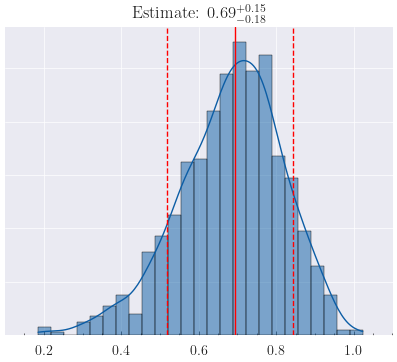
\includegraphics[width=\textwidth]{img/chao1boot.png}
		\caption{Chao1}
		\label{fig:chao1}
	\end{subfigure}
	\hfill
	\begin{subfigure}[b]{0.32\textwidth}
		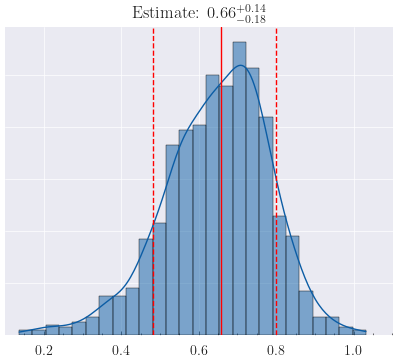
\includegraphics[width=\textwidth]{img/ichaoboot.png}
		\caption{iChao1}
		\label{fig:ichao1}
	\end{subfigure}
	\hfill
	\begin{subfigure}[b]{0.32\textwidth}
		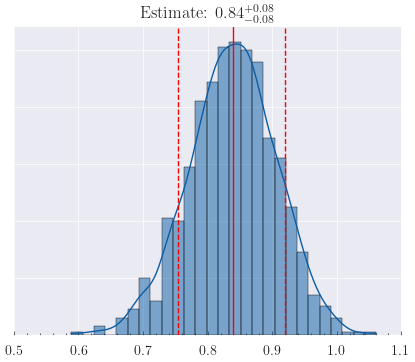
\includegraphics[width=\textwidth]{img/aceboot.png}
		\caption{ACE}
		\label{fig:ace}
	\end{subfigure}
	
	\caption{\textbf{Estimations et variabilité des taux de survie des textes par les estimateurs de richesse via méthode de  \textit{bootstrap} : Chao1, iChao1 et ACE}}
	
	\label{fig:estimators}
\end{figure}

Ces trois courbes de densité représentent une estimation des taux de survie des textes. Il en ressort à nouveau que les estimateurs de richesse Chao1 et iChao produisent des résultats très proches : ils estiment respectivement que 69 \% et 66\% des textes des Pères de l'Église en péninsule Ibérique ont survécu. Toutefois, bien que ces estimations soient proches, une incertitude non négligeable demeure : leurs intervalles de confiance sont quasiment similaires, allant de -0,18 à +0,15 pour Chao1, et de -0,18 à +0,14 pour iChao. L’estimation d’ACE est quant à elle plus élevée, puisqu’elle donne un taux de survie des œuvres de 80 \%. L’intervalle de confiance est également plus resserré, puisqu’il est compris entre -0,08 et +0,08. Néanmoins, il convient de garder à l'esprit que, bien que les estimations de la richesse spécifique obtenues par la méthode bootstrap appliquée à l'estimateur ACE présentent une incertitude réduite, cet estimateur demeure particulièrement sensible à un hyperparamètre, \textit{k}, définissant le seuil des espèces rares, comme nous l’avons souligné précédemment. Ces résultats doivent donc être interprétés avec prudence.

Grâce à la méthode \texttt{Minsample}, nous pouvons également obtenir une estimation du taux de survie des manuscrits qui ont transmis les textes des Pères de l'Eglise en péninsule Ibérique:

\begin{figure}[H]
	\centering
	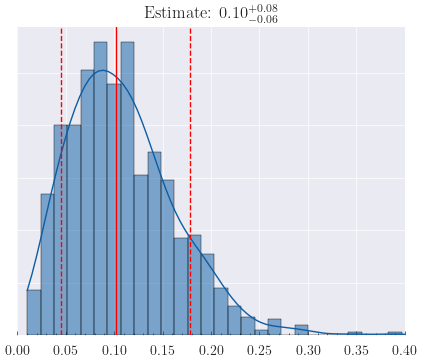
\includegraphics[width=0.7\textwidth]{img/minsampleboot.png}
	\caption{\textbf{Estimation et variabilité du taux de survie des manuscrits via méthode de \textit{bootstrap} }}
	\label{fig:ton_label}
\end{figure}
	
Comme le montre le graphique, seuls 10\% des témoins contenant les textes patristiques de la péninsule Ibérique ont été conservés, avec un intervalle de confiance de -0,06 à +0,08.  \newpage


Pour conclure, notre corpus semble être au prise d'une tendance antagoniste : alors qu'une grande majorité des textes semble avoir survécu, seulement une minorité de témoins nous sont parvenus. Ces résultats doivent cependant être interprétés avec précaution. Au-delà des incertitudes associées aux estimateurs eux-mêmes, une autre source de fragilité réside dans notre corpus qui représente une petite population.  Cela se traduit avant tout par l'aspect de nos courbes de densité : elles sont peu lisses et nous pouvons même noter la présence d’artefacts, en particulier dans les queues des distributions. Néanmoins, les ordres de grandeur obtenus apportent des premiers éléments utiles à la réflexion sur la survie des textes des Pères de l’Église en péninsule Ibérique. Ils ne sauraient être tenus pour définitifs et un élargissement du corpus constituerait une piste essentielle pour affiner ces estimations et en améliorer la fiabilité. \newpage

\section {La courbe d'accumulation des espèces}

Une autre manière de décrire la diversité en biologie est de construire une courbe d'accumulation des espèces: elle représente « le nombre d'espèces découvertes en fonction de l'effort d'échantillonnage »\footnote{Définition extraite du dépôt GitHub \textit{MesuresBioDiv2} d’Éric Marcon, section \textit{Outils}, disponible à l’adresse \url{https://github.com/ericmarcon/MesuresBioDiv2}.}. Ce qui est représenté est donc l'effet statistique de l'échantillonnage.

Dans le logiciel \textit{Copia}, c'est la fonction \texttt{accumulation\_curve} qui permet de tracer cette courbe: \\

\begin{figure}[H]
	\centering
	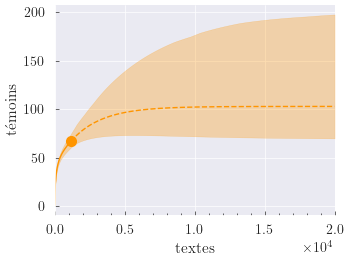
\includegraphics[width=0.8\textwidth]{img/accumulation.png}
	\caption{\textbf{Courbe d'accumulation des espèces. }}
	Le point orange représente les données empiriques, la courbe pleine correspond à la courbe de raréfaction, la courbe en pointillés est la courbe d’extrapolation, et la zone orange illustre l’aire d’incertitude.
	\label{fig:ton_label}
	\end{figure}


Le point orange correspond à nos données empiriques : nous disposons de 67 textes observés pour un total de 1159 témoins. La courbe se lit dans les deux directions : d’un côté, l’extrapolation (courbe en pointillés) fournit une estimation numérique du nombre d’espèces supplémentaires que l’on pourrait découvrir en augmentant la taille de l’échantillon. Concrètement, dans notre cas, cette extrapolation indique combien de nouveaux manuscrits, par exemple issus de collections privées encore inexplorées, il faudrait découvrir pour espérer révéler un ou plusieurs textes actuellement inconnus. Dans l’autre sens, la courbe pleine traduit le phénomène inverse, appelé raréfaction : elle estime théoriquement le nombre d’espèces que l’on aurait observé si la taille de l’échantillon avait été inférieure à celle réellement analysée. L’aire en orange clair autour de la courbe matérialise l’incertitude associée à cette estimation, qui demeure importante compte tenu de la taille limitée de notre population. Malgré cette incertitude, l’interprétation reste possible : lorsque la pente de la courbe tend vers zéro, autrement dit lorsque celle-ci s’aplatit, cela signifie que l’on ne s’attend plus à découvrir de nouveaux textes en augmentant l’échantillonnage. Autrement dit, nous avons approché la richesse spécifique totale du corpus, ayant échantillonné la quasi-totalité des espèces.

Afin de localiser précisément l’endroit où la courbe commence à tendre vers zéro, nous avons implémenté une fonction appelée \texttt{detect\_flattening}. Celle-ci analyse à chaque nouveau point de la courbe comment la richesse spécifique (le nombre de textes distincts) évolue en fonction du nombre de témoins considérés. Concrètement, cela revient à calculer la variation entre chaque point consécutif de la courbe. Nous avons fixé un seuil à 0.001 : lorsque la courbe atteint ou passe en dessous de ce seuil, elle cesse de croître de manière significative. Cela indique que nous sommes dans une zone de stagnation : même si de nouveaux témoins sont découverts, ils n’apportent plus de nouveaux textes.

\begin{figure}[H]
	\centering
	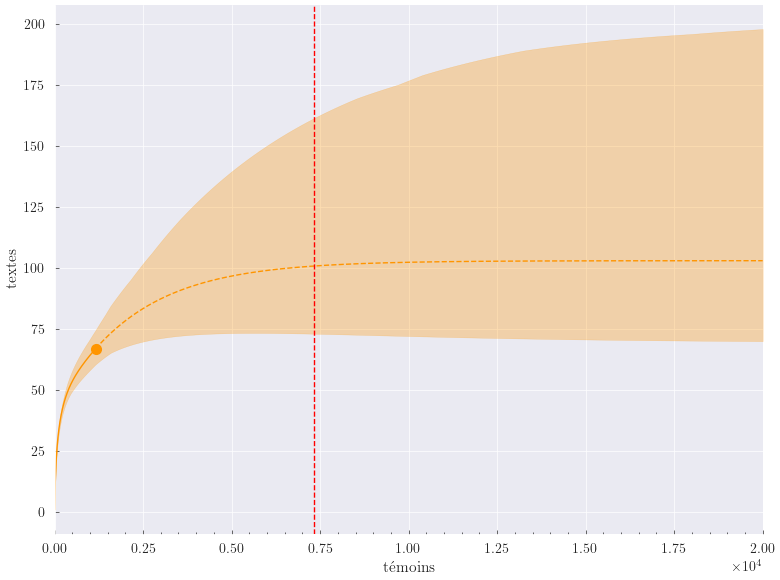
\includegraphics[width=0.8\textwidth]{img/applatissement.png}
	\caption{\textbf{Détection du point de saturation de la courbe d'accumulation des espèces }}
	 Le point orange représente les données empiriques, la courbe pleine correspond à la courbe de raréfaction, la courbe en pointillés est la courbe d’extrapolation, et la zone orange illustre l’aire d’incertitude. La ligne rouge en pointillés indique le point à partir duquel la courbe commence à s’aplatir, suggérant un ralentissement de la découverte de nouvelles espèces.
	 
	\label{fig:ton_label}
\end{figure}

Notre fonction \texttt{detect\_flattening} indique que la courbe d'accumulation passe en dessous du seuil de 0{,}001 à partir de 7314 témoins. Cela signifie qu’au-delà de ce point, l’ajout de nouveaux témoins n’entraîne plus la découverte de textes inédits des Pères de l’Église en péninsule Ibérique.


\section{Le nombre de Hill}

Le nombre de Hill est l'un des indices de diversité. Un indice de diversité consiste à mesurer la diversité d'une communauté en tenant compte à la fois du nombre d'espèces et de leur abondance relative. Les trois indices de diversité les plus courants sont ceux de Shannon-Weaver, Simpson et Hill. L'indice de Hill incluant les deux premières indices, nous rappelons brièvement leur principe\footcite[Pour les définitions des indices de diversité, nous nous sommes appuyés sur le cours d'Eric Marcon, chercheur en écologie tropicale à l’UMR Amap et enseignant à AgroParisTech. Le cours est disponible sur : ][chapitre Entropie]{MarconMesuresBioDiv2} :

\paragraph{Indice de Shannon-Weaver}

Sa formule calcule pour chaque espèce la proportion d’individus qu’elle représente dans le total (\(N_i / N\)). On constate que cette proportion est multipliée par le logarithme de cette même proportion. Le logarithme sert à donner plus de poids aux espèces rares et moins aux espèces très communes, ce qui rend notre indice plus sensible à la diversité réelle. Le signe négatif en début sert à transformer l’indice, qui serait négatif, en un indice positif : en effet, l’utilisation du logarithme donne toujours des valeurs négatives ou nulles. \\

$H' = - \sum_{i=1}^{S} \left( \frac{N_i}{N} \times \log_2 \frac{N_i}{N} \right)$\\

\begin{itemize}
	\item $N_i$ : nombre total d’individus de l’espèce $i$.
	\item $N$ : nombre total d’individus toutes espèces confondues.
	\item $S$ : nombre total d’espèces.
\end{itemize}

\paragraph{Indice de Simpson}

L'indice de Simpson adopte quant à lui une toute autre stratégie de calcul de la diversité :  il repose sur la probabilité que deux individus pris aléatoirement dans l'échantillon soit de la même espèce. Pour se faire, on regarde pour chaque espèce combien de paires elle peut former avec les individus puis on divise la somme de ces paires  par le nombre total de paires possibles dans tout le groupe : \\

$D = \sum_{i=1}^{S} \frac{N_i (N_i - 1)}{N (N - 1)}$ \\

\begin{itemize}
	\item $N_i$ : nombre total d’individus de l’espèce $i$.
	\item $N$ : nombre total d’individus toutes espèces confondues.
	\item $S$ : nombre total d’espèces.
\end{itemize}

\paragraph {Indice de Hill}

L'indice de Hill est le plus précis car il intègre les deux autres indices, Shannon\-Weaver et Simpson. En voici la formule, telle qu'elle est implémentée dans le logiciel \textit{Copia}: \\

$D_q = \left( \sum_{i=1}^{S} p_i^q \right)^{\frac{1}{1 - q}}, \quad \text{pour } q \neq 1$\\

\begin{itemize}
	\item $D_q$ : nombre de Hill pour un paramètre de sensibilité $q$.
	\item $S$ : nombre total d’espèces dans l’échantillon.
	\item $p_i$ : proportion d’individus appartenant à l’espèce $i$.\\
\end{itemize} 

Pour $q = 1$, il est nécessaire de rajouter une limite car à l'exposant on obtient une forme \(\frac{0}{0}\) puisque l’exposant est \(\frac{1}{1-1} = \frac{1}{0}\), ce qui est infini. Nous en déduisons que c'est pour cela que dans la fonction \texttt{compute\_empirical\_hill\_numbers} de \textit{Copia} une limite a été implémentée pour $q = 1$ :

\[
\lim_{q \to 1} \left( \sum_{i=1}^S p_i^q \right)^{\frac{1}{1-q}} 
= \exp\left(- \sum_{i=1}^S p_i \log p_i \right)
\]\\

\begin{itemize}
	\item \(p_i\) : proportion d’individus appartenant à l’espèce \(i\).
	\item \(S\) : nombre total d’espèces.
	\item \(q\) : paramètre d’ordre des nombres de Hill.\\
\end{itemize}


Le principe de cette mesure, comme nous l'avons précisé est d'intégrer d'autres indices. Cela est permis grâce au paramètre \textit{q}. En changeant sa valeur, la formule « change » et donne les mêmes résultats que les indices de Shannon-Weaver et Simpson pour respectivement \( q = 1\) et \( q = 2 \).
Quand \( q = 0 \), on obtient la richesse spécifique. En effet, dans la formule, on élève chaque proportion \( p_i \) à la puissance 0. Or, n’importe quel nombre (sauf zéro) à la puissance 0 vaut 1. Donc, on compte juste le nombre d’espèces qui ont au moins un individu, ce qui revient à la richesse spécifique. Ainsi, quand  \( q = 0 \) on obtient seulement le nombre d'espèces différentes, sans prendre en compte le nombre d'individus.
Quand \( q = 1 \), la formule reprend le principe de la formule de Shannon-Weaver. On a vu qu'avec  \( q = 1\), on ajoute une limite. On constatera que cette dernière est la formule de Shannon-Weaver à l'exponentielle.
 Pour \( q = 2 \), on calcule la somme des carrés des proportions des espèces (\( p_i^2 \)). Puis on prend l'inverse de la somme des carrés des proportions puisque l’exposant \(\frac{1}{1 - q}\) avec \(q = 2\)    devient \(-1\). On se rend compte que cette formule est l'inverse de l'indice de Simpson. Ainsi, on remarque que le paramètre \textit{q} dans la formule de l’indice de Hill fait varier l’importance relative accordée aux espèces fréquentes et rares. Lorsque \( q = 0 \), chaque espèce compte autant, qu’elle soit très fréquente ou presque absente, puisqu’on mesure simplement la richesse spécifique. Lorsque \( q = 1 \), l’effet des espèces fréquentes et rares est pris en compte mais de façon compensée grâce à l’utilisation du logarithme. En revanche, pour \( q = 2 \), l’effet est inversé : l’élévation au carré accentue les écarts entre les proportions. Les grandes proportions deviennent encore plus importantes, tandis que les petites deviennent quasiment négligeables.
 Une dernière remarque est que lorsque nous calculons la diversité avec les indices de Shannon-Weaver ou de Simpson, les valeurs obtenues sont souvent difficiles à interpréter directement : par exemple, que signifie un indice de Shannon-Weaver égal à 1,5 ? C'est pourquoi l'indice de Hill applique des transformations, comme l’exponentielle pour Shannon ou l’inverse du carré pour Simpson afin de rendre ces indices plus intelligibles. Ainsi, on obtient ce qu’on appelle un nombre effectif d’espèces, qui diffère du simple nombre brut d’espèces. Ce nombre effectif correspond au nombre d’espèces également abondantes qu’il faudrait avoir pour obtenir la même diversité que celle observée.
Pour résumer, l’indice de Hill est une mesure de diversité qui intègre différents indices classiques (comme Shannon ou Simpson) en les transformant pour qu’ils deviennent plus facilement interprétables. Grâce au paramètre \( q \), on peut ajuster la sensibilité de la mesure aux espèces rares ou fréquentes, ce qui permet d’obtenir un nombre effectif d’espèces reflétant mieux la diversité réelle de la communauté étudiée.

 
 
Le logiciel \textit{Copia} permet d'appliquer l'indice de Hill sur nos données empiriques mais également sur celles corrigées des biais liés aux espèces non observées (par exemple avec la méthode de Chao1, présentée précédemment)\footnote{Pour cette méthode, se référer au fichier \texttt{diversity.py} du dépôt GitHub de \textit{Copia}, disponible à l'adresse \url{https://github.com/mikekestemont/copia}}. On obtient alors une courbe représentant la formule de l'indice de Hill pour tout  $q \geq 0$:

\begin{figure}[H]
	\centering
	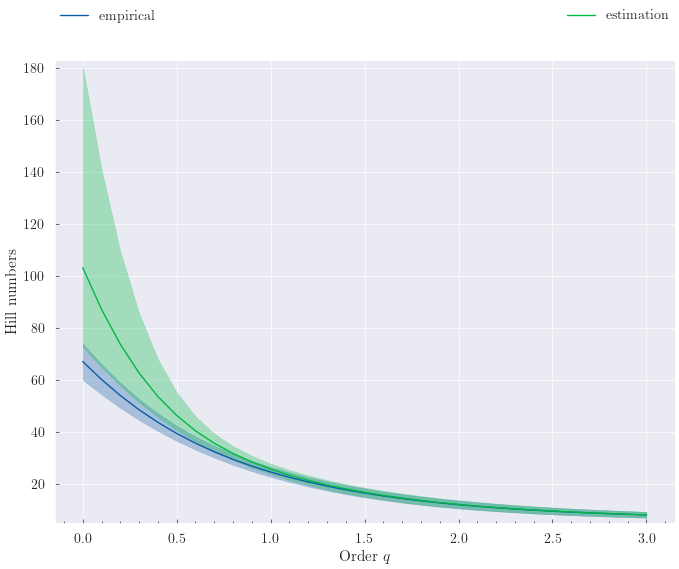
\includegraphics[width=0.8\textwidth]{img/hillnumber.png}
	\caption{\textbf{Diversité selon l’indice de Hill}}
	La courbe bleue représente l'indice de Hill empirique, la courbe verte l'indice de Hill estimé,
	et les zones bleue et verte indiquent les incertitudes associées à chaque courbe.	
	\label{fig:ton_label}
\end{figure}

\paragraph{Application de l'indice de Hill sur nos données empiriques} Pour \( q = 0 \), on souligne que le nombre d'espèces est exactement celui observé dans nos données soit 67 textes différents. La courbe observée sur notre graphique est strictement décroissante. Lorsque \( q > 0 \), on rappelle que les nombres de Hill fournissent une mesure pondérée de la diversité. Par exemple, à \( q = 1 \), on obtiendrait l’équivalent de 25 espèces également abondantes. À \( q = 1{,}5 \), ce nombre effectif descend à 17, puis à 14 pour \( q = 2 \). Cette valeur continue de diminuer jusqu’à \( q = 3 \), où l’on aurait à peine l’équivalent de 3 espèces abondantes. Cette diminution stricte traduit donc une forte inégalité dans les abondances : la diversité n’est pas répartie équitablement entre toutes les espèces, mais dominée par un petit nombre d’espèces majoritaires. En d'autres termes, bien que 67 textes différents soient présents, la diversité effective est beaucoup plus faible, car la majorité des témoins se concentrent sur un nombre réduit de textes.

\paragraph{Application de l'indice de Hill sur nos données corrigées des biais liées  aux espèce observées} La courbe est aussi strictement décroissante et rejoint rapidement celle des données empiriques, dès \( q = 1{,}2 \). À \( q = 0 \), on estime la richesse spécifique à 103 espèces, ce qui correspond à la valeur de l’estimateur Chao1. Pour \( q = 1 \) et \( q = 2 \), correspondant aux indices de Shannon-Weaver et de Simpson comme expliqué plus tôt, le nombre effectif d’espèces est très proche de celui des données empiriques : 25 espèces contre 27 à \( q = 1 \), et 14 espèces pour les deux à \( q = 2 \).
Cet ajustement rapide entre les deux courbes peut s'expliquer par le fait que quand le paramètre \textit{q} est proche de 0, on considère toutes les espèces de manière équivalentes, que celles-ci soient 
abondantes ou rares. Mais quand \textit{q} augmente, on tient de plus en plus compte des espèces abondantes qui sont généralement bien représentées dans les données empiriques, contrairement aux espèces rares qui ont tendance à être sous-échantillonnées. La diversité empirique et estimée deviennent dès lors très proches.

\section{L'équitabilité}

L'équitabilité se définit par « l'écart entre la distribution observée et une distribution uniforme »\footcite[chapitre Equitabilité]{MarconMesuresBioDiv2}. On analyse ainsi dans quelle mesure les espèces ont des abondances proches ou déséquilibrées. Cette mesure est  importante à prendre en compte dans notre cas : si notre communauté de textes est très déséquilibrée, cela signifie que certains textes disposent de nombreux témoins tandis que d'autres ne sont conservés que par un seul. Dans ce contexte, on est beaucoup plus susceptibles de perdre un texte lors d’événements destructeurs comme des incendies de bibliothèques ou des guerres. En revanche, pour les textes très bien attestés, la perte de quelques témoins n’empêchera pas leur transmission.

Dans le logiciel \textit{Copia}, l’équitabilité est représentée par la fonction \texttt{compute\_evenness}, qui calcule un profil d’équitabilité à partir des nombres de Hill. On utilise ces indices car, comme indiqué précédemment, ils offrent plusieurs perspectives de la diversité selon le paramètre \textit{q}. En se basant sur ce profil de diversité pour différentes valeurs de \textit{q}, la fonction génère alors un profil d’équitabilité.


\begin{figure}[H]
	\centering
	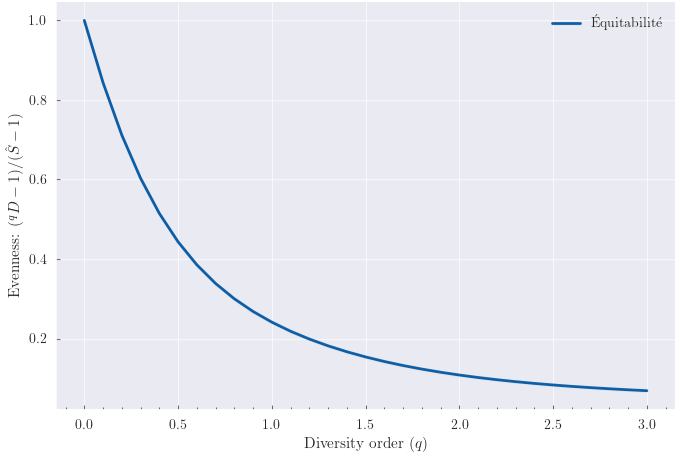
\includegraphics[width=0.8\textwidth]{img/evenness.png}
	\caption[\textbf{Profil d’équitabilité en fonction de l’ordre \(q\)}]{%
		Profil d’équitabilité en fonction de l’ordre \(q\) de 0 à 3. 
		L’axe des abscisses correspond à l’ordre de diversité \(q\), variant de 0 à 3, qui permet de moduler la sensibilité de la mesure aux espèces rares ou abondantes. L’axe des ordonnées montre l’équitabilité, calculée comme 
		$\frac{{}^q D - 1}{\hat{S} - 1}$,
		où \({}^q D\) est le nombre de Hill d’ordre \(q\) et \(\hat{S}\) la richesse totale. Cette valeur, comprise entre 0 et 1, mesure l’uniformité de la distribution des espèces. 
	}
	\label{fig:ton_label}
\end{figure}


La courbe du profil d’équitabilité pour les textes patristiques en péninsule Ibérique est strictement décroissante. Le raisonnement est similaire à celui appliqué à l’indice de Hill : à \( q = 0 \), l’équitabilité est élevée car elle intègre à la fois les espèces rares et abondantes. Cependant, à mesure que \( q \) augmente, on accorde de plus en plus de poids aux espèces abondantes. Cela reflète une répartition très inégale, où quelques espèces dominent largement l’assemblage, ce qui réduit l’équitabilité globale. 

\section{Conclusion partielle}

Ces différentes analyses fournissent une première évaluation quantitative du degré de perte au sein de notre corpus patristique de la péninsule Ibérique, en mobilisant des outils empruntés à l’écodiversité. Les estimateurs de richesse appliqués à notre échantillon (malgré des incertitudes notables et une sensibilité marquée à certains paramètres) convergent vers une estimation minimale comprise entre 100 et 110 textes disparus et 14774 témoins disparus. Ces méthodes s’appuient sur la rareté textuelle, c’est-à-dire sur la présence de textes ayant seulement quelques témoins qui ont survécu, ce qui constitue un indicateur fort de lacunes potentielles dans la transmission manuscrite. La courbe d’accumulation des espèces vient renforcer cette lecture en proposant une représentation visuelle de la dynamique de découverte des textes : elle montre que la probabilité de mettre au jour de nouveaux textes diminue sensiblement au-delà d’un certain seuil d’échantillonnage. Dans notre cas, ce point d’inflexion se situe à 7314 témoins, au-delà duquel l’ajout de nouveaux témoins devient statistiquement peu susceptible de révéler des textes inédits.
Enfin, l’analyse des indices de Hill et du profil d’équitabilité met en lumière un déséquilibre structurel au sein de notre corpus : certains textes ont été largement diffusés tandis que d'autres n'ont survécu que par quelques témoins. Si l'on associe cette analyse à celle menée empiriquement sur les données d'abondance, on peut affirmer que ce sont quelques textes poétiques, très largement copiés et surreprésentés, qui concentrent à eux seuls la majeure partie des témoins. Ce déséquilibre marqué nous renvoie au fait que notre tradition patristique est fragile : au cours du temps, plusieurs textes ont pu disparaitre car ils n'étaient pas transmis par un nombre de témoins suffisant.


\part{ À la recherche du manuscrit perdu : parcours stochastiques d’un texte}

\chapter{Approches stochastiques de la transmission}

Notre dernière analyse consistera à appliquer à nos données une méthode fondée sur des modèles stochastiques de type naissance-mort, couplés à des simulations informatiques. Nous avons vu que l'application de processus de naissance et de mort pour représenter les dynamiques de transmission des manuscrits et des textes avait déjà été proposée le siècle dernier par M. P.~ Weitzman\footcite{weitzman1987evolution}. Cette approche, reprise récemment dans l'article « Lost manuscripts and extinct texts : A dynamic model of cultural transmission »\footcite{Camps2022} de J-B. Camps et J. Randon-Furling, est actuellement approfondie dans le cadre du projet \textit{ERC-LostMA}, lancé en 2024\footnote{Pour suivre les avancées du projet, voir \url{https://lostma-erc.github.io/about}.}.

Contrairement aux méthodes classiques d’estimation, comme celles des espèces non vues, cette approche se concentre sur la modélisation dynamique du phénomène de transmission : en effet, elle permet de décomposer ce dernier en simulant l’évolution de la population des textes et des témoins au fil du temps. L’objectif serait ainsi de retracer les processus évolutifs ayant conduit à la constitution de notre corpus actuel (en d’autres termes, les dynamiques de préservation, de copie et d’extinction des œuvres manuscrites, qui expliquent pourquoi seuls 67 textes et 1159 témoins nous sont parvenus). 

%Les données mobilisées seront de deux types : comme pour la méthode des espèces non vues, nous avons besoin de données d’abondance (nombre de témoins, nombre de textes, etc.). Mais cette méthode requiert également, lorsqu'ils ont été tracés, les \textit{stemmata codicum} des œuvres étudiées.

%

\section{Processus de naissance et de mort}

\subsection{En quoi ce modèle est-il applicable au phénomène de transmission textuelle et manuscrite?}

Une première manière de modéliser les dynamiques de population des manuscrits et des textes patristiques consiste à utiliser un processus stochastique simple de type naissance et mort. En simplifiant au maximum le phénomène de transmission textuelle, on peut considérer que chaque manuscrit appartient à une population qui évolue selon deux seules issues possibles : soit il est copié et donc survit, soit il disparaît. Cette dynamique de préservation ou d’extinction peut résulter de multiples facteurs, qu’ils soient naturels (incendies, guerres, dégradations matérielles) ou humains (désintérêt progressif pour une œuvre, succès entraînant une large diffusion par copie). La transmission des textes repose ainsi essentiellement sur deux mécanismes : la copie et la perte. Mathématiquement, ce phénomène culturel peut être modélisé par un processus stochastique de type naissance et mort. Nous n'entrerons pas dans tous les détails techniques de la méthode, largement expliquée dans l’article de référence\footcite{camps_transmission_2025}. Nous nous contenterons d'en présenter les grands principes et la logique afin que notre lecteur puisse comprendre la démarche.

La modélisation stochastique vise essentiellement à « préciser des lois de probabilité qui rendent compte des variations aléatoires observées dans certains phénomènes, ces variations résultant de causes soit inconnues, soit impossibles à mesurer ». Elle trouve une application notable dans le domaine financier, où elle sert à prévoir l’évolution des cours en bourse\footcite{Cunchala}, mais aussi en biologie, notamment pour étudier la génétique des populations et modéliser l’évolution aléatoire des allèles d’une génération à l’autre\footcite{Elowitz}. Un type particulier de modèle stochastique est celui qui repose sur un processus de Markov : en résumé, la probabilité d’un événement futur dépend uniquement de l’état présent, sans tenir compte de l’historique passé du phénomène. Le processus de naissance et de mort constitue alors un cas spécifique de ce type de processus.\footnote{Ces définitions sont tirées d’un cours en ligne très accessible: \url{https://dept-info.labri.fr/ENSEIGNEMENT/formation-a-distance/cibermiage-processus/c1.7/accueil.htm}.}


 Un processus est dit de type naissance-mort s’il satisfait plusieurs conditions\footnote{Ces conditions sont établies d’après le manuel \textit{Essentials of Stochastic Processes} de Richard Durrett \cite{durrett2016essentials}.}:

\begin{itemize}
	\item La population doit évoluer par des changements discrets : cela correspond bien à nos manuscrits, puisqu’ils sont des valeurs entières. Par exemple, il est impossible d’obtenir 1{,}5 manuscrits.
	\item Les probabilités de naissance et de mort dépendent seulement de l’état actuel du processus : cela convient à notre population de manuscrits car leur évolution à chaque pas de temps dépend uniquement du nombre actuel de manuscrits.
	\item Les taux de naissance et de mort doivent être non négatifs : notre population de manuscrits répond également à cette dernière condition puisqu'un manuscrit ne peut qu'avoir une probabilité positive ou nulle d'être copié.
\end{itemize}

Une fois ces conditions remplies, le principe est le suivant : chaque manuscrit peut, à chaque instant, soit être copié (ce qui correspond à une « naissance »), soit disparaître (une « mort »), selon deux paramètres : le taux de copie, noté $\lambda$, et le taux de perte, noté $\mu$. Ainsi, la population des manuscrits évolue dans le temps : à chaque pas de temps, chaque manuscrit peut être recopié ou perdu, en fonction de ces deux probabilités.

Le modèle de naissance-mort permet donc de simuler de manière probabiliste l’évolution d’une tradition avec ses dynamiques de préservation ou d'extinction des manuscrits. Mais ce modèle a besoin d'être paramétré, et dans la réalité, on ne connaît pas directement ces paramètres: on observe uniquement l’état final du corpus (par exemple, le nombre de textes conservés et le nombre de manuscrits qui ont survécu). 

\subsection{Deux stratégies : exploration empirique et inférence}

Une première stratégie, adoptée dans les travaux déjà énoncés de J.-B Camps et \textit{al.}\footcite{Camps2022, camps_transmission_2025} consiste à explorer des plages de valeurs pour les paramètres du modèles à partir d’hypothèses issues du savoir philologique et historique. Cette étude a récemment été complétée par une autre approche : l’inférence. Pour notre étude, nous avons choisi d’adopter cette dernière : il s’agit pour nous de déterminer, par inférence, les paramètres les plus pertinents pour représenter notre tradition de textes patristiques. Nous nous appuierons pour cela sur les travaux réalisés dans le dépôt \textit{SimMAtree} du projet \textit{LostMA} \footcite{simmatree_github}, où un algorithme d’inférence bayésienne a été appliqué à des données de distribution de témoins à l’aide d’un processus de naissance-mort de type Poisson ou Yule. Comme à d’autres endroits dans ce travail, nous optons ici pour une présentation simplifiée de l’inférence bayésienne. Les lecteurs désireux d’approfondir les aspects mathématiques du fonctionnement de cette méthode, notamment dans le cadre de la transmission textuelle, sont invités à consulter directement le dépôt GitHub du projet. Pour une vue d’ensemble plus théorique, accompagnée de cas d’usage variés, le \textit{Handbook of Approximate Bayesian Computation} constitue une référence utile\footcite{sisson}. Le principe de l'inférence bayésienne est le suivant : on cherche à retrouver les paramètres les plus probables à partir des données observées. Dans l'idée,  un  algorithme génère un grand nombre de simulations du modèle avec des couples de paramètres tirés aléatoirement, puis compare les sorties simulées aux données réelles. L’algorithme apprend alors à estimer la distribution des paramètres les plus compatibles avec les observations. En se permettant une réflexion d’ordre presque philosophique, on pourrait dire que le cœur de l’inférence bayésienne consiste à mettre à jour nos croyances sur les paramètres après confrontation aux données observées. Nous partons avec une idée préalable, un \textit{a priori} sur ces paramètres, et le processus d'inférence bayésienne nous aide à repositionner cette croyance à la lumière des estimations faites sur nos données.




\subsubsection{Ajustement des paramètres}

Nous avons tout d'abord choisi d’appliquer l’inférence au modèle \texttt{BirthDeathPoisson} proposé dans \textit{SimMAtree}. Il s’agit du modèle stochastique simple de type naissance-mort, tel que présenté plus haut, dans lequel les deux principaux paramètres à estimer sont $\lambda$ (le taux de naissance) et $\mu$ (le taux de mort) des manuscrits. Pour faire tourner notre modèle via inférence bayésienne, certains hyperparamètres doivent être définis en entrée : on doit fixer un nombre de population initiale ($n_{\text{init}}$), un maximum de population ($\text{max\_pop}$) qui représente en quelque sorte une limite que notre population de témoins ne peut pas dépasser mais aussi déterminer des périodes de temps.


Le modèle stochastique de processus de naissance et de mort, tel qu’il est présenté dans l’article « On the transmission of texts: written cultures as complex systems »\footcite{camps_transmission_2025}, a été appliqué à un corpus de récits de chevalerie autour des figures de Charlemagne et d’Arthur, diffusés à travers l’Europe entre le XII\textsuperscript{e} et le XIV\textsuperscript{e} siècle. Notre corpus s'en distingue nettement : il concerne une tradition d’un tout autre type, celle des Pères de l'Eglise, dans un contexte chronologique différent, l’Antiquité tardive, et se limite géographiquement à la seule péninsule Ibérique. 

Ces différences géographiques et chronologiques justifient le fait que nous ne pouvons pas réutiliser les mêmes hyperparamètres que ceux employés dans l'étude de J. B. Camps et \textit{al.}\footcite{camps_transmission_2025}. Nous devons les adapter aux spécificités de notre corpus. L’un des ajustements les plus importants a concerné la définition des périodes de temps. En effet, le modèle stochastique de processus de naissance et de mort de transmission textuelle repose sur un découpage temporel en  deux phases distinctes : une période d’activité et une période d’inactivité. La première correspond au moment où les textes étaient activement copiés, la seconde à celui où ils ne l’étaient plus, mais continuaient néanmoins à circuler ou à être conservés. Plus précisément, ces hyperparamètres de temps ont été établis comme suit, en suivant la démarche de l'article de référence pour cette approche\footcite{camps_transmission_2025} : la période active débute à la fin du III\textsuperscript{e} siècle (vers 300), date estimée des premières œuvres de notre corpus, et s’étend jusqu’au XVe siècle (environ 1450), soit jusqu’à l’invention de l’imprimerie. Cela représente une durée d’environ 1150 ans. La période inactive couvre ensuite la Renaissance jusqu’au début de la Révolution industrielle (environ 1450 à 1800), soit 350 ans.
Conformément à la logique du modèle, chaque pas de temps dans la simulation correspond à un trimestre (soit 0{,}25 an).\footnote{Ce pas de temps a été défini à partir d’une estimation basée sur des données historiques concernant le temps moyen nécessaire à un copiste pour réaliser 200 pages. Pour plus de détails, voir la section \textit{Methods} de l’article « On the transmission of texts: written cultures as complex systems » de J.-B Camps, J. Randon-Furling et U. Godreau.
} Nous avons donc défini une durée de 4600 pas pour la période active ($1150 \div 0{,}25$) et de 1400 pas pour la période inactive ($350 \div 0{,}25$), pour un total de 6000 pas, équivalant à 1500 ans. Ce découpage permet de rendre compte au plus près de la temporalité spécifique à notre tradition. Ainsi, on souligne que la période de copie et de circulation des manuscrits de notre corpus s’étale sur une durée nettement plus longue que celle des récits de chevalerie médiévaux. Cette période de temps étirée augmente donc logiquement les probabilités de perte de certains manuscrits ou textes au fil du temps. 

\subsection{Résultats de l'inférence bayésienne sur nos données modélisées à l’aide d’un processus de naissance-mort de type Poisson}

Nous avons fait tourner 30000 simulations, chacune basée sur 15000 échantillons. Les hyperparamètres ont été réglés de la sorte: \begin{itemize}
	\item \textbf{Modèle} : \texttt{BirthDeath}
	\item \textbf{Paramètres} :
	\begin{itemize}
		\item \texttt{n\_init} = 500
		\item \texttt{Nact} = 4600
		\item \texttt{Ninact} = 1400
		\item \texttt{max\_pop} = 300000\footnote{En ce qui concerne l’hyperparamètre \( n_{\text{init}} \) et max\_pop, nous les avons fixés à 500 et 300000 par défaut. À ce jour, aucune donnée historique ni indication philologique ne permet d’en proposer une estimation plus rigoureuse.
		}
	\end{itemize}
\end{itemize}


\begin{figure}[H]
	\centering
	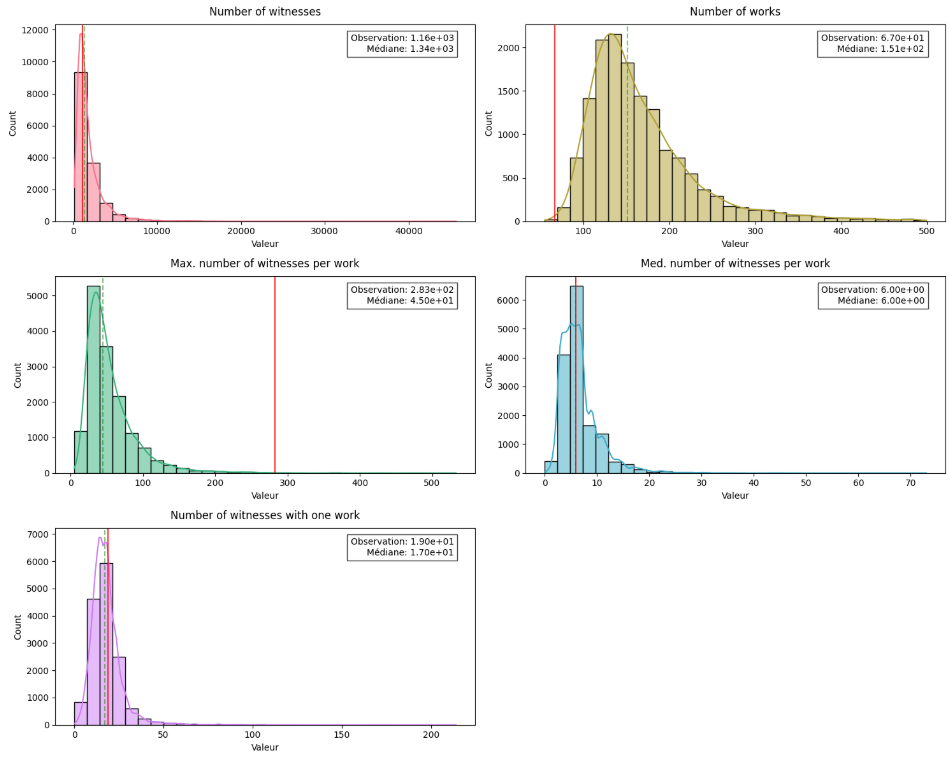
\includegraphics[width=0.9\textwidth]{img/simus_plot.png}
	\caption{\textbf{Comparaison entre les données simulées et observées issues de l’inférence bayésienne.}}
	\label{fig:fig_simus}
\end{figure}

L’inférence s’avère globalement satisfaisante pour certaines statistiques clés, notamment le nombre total de témoins, la médiane du nombre de témoins par texte et le nombre de singletons. Nos données empiriques comptent 1159 témoins, tandis que la médiane des simulations en produit 1340, ce qui est relativement proche. De même, pour les singletons, nous en observons 19 dans le corpus réel, contre une médiane simulée de 17, là encore dans un ordre de grandeur comparable. C'est au niveau de la médiane du nombre de témoins par texte que nous obtenons le résultat le plus probant, avec une médiane identique de 6 témoins par texte. En revanche, pour le nombre de textes, notre simulation a tendance à surestimer la réalité : nos données empiriques contiennent 67 textes alors que nous avons 151 textes en moyenne dans les données simulées. L’inférence ne parvient également pas à reproduire correctement le nombre maximal de témoins par texte, estimé à 45 par les simulations, alors qu’il atteint 283 dans notre corpus.

Les résultats de l’inférence permettent également de visualiser les corrélations entre les différents paramètres du modèle. Parmi celles-ci, nous nous concentrerons sur$\lambda$ et $\mu$, qui sont les deux paramètres principaux. Il se trouve qu'ils apparaissent nettement corrélés l’un à l’autre.

\begin{figure}[H]
	\centering
	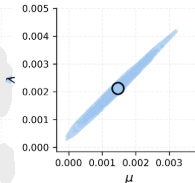
\includegraphics[width=0.7\textwidth]{img/correlationlm.png}
	\caption{\textbf{Relation entre les paramètres $\lambda$ (taux de copie) et $\mu$ (taux de perte) après inférence.}}
	\label{fig:fig_simus}
\end{figure}

La forme elliptique croissante observée entre $\lambda$ et $\mu$ dans les graphiques de corrélation traduit une relation positive entre ces deux paramètres : Plus certaines copies tendent à disparaître, plus d’autres sont reproduites en grand nombre. Cette dynamique s’explique par la structure même de notre corpus, qui comporte un nombre total de témoins très élevé (1159 pour 67 textes), une forte disparité dans la diffusion des textes (avec un maximum de 283 témoins pour un seul texte), ainsi qu’un nombre non négligeable de singletons (19 textes n’ayant qu’un seul témoin). Ce profil très asymétrique contraint le modèle à trouver un équilibre entre perte et copie : un taux de perte élevé ne peut engendrer une telle densité de transmission sans une augmentation correspondante du taux de copie. Ainsi, il semble que la distribution de nos données en queue lourde explique cette forte corrélation entre les taux de perte et de survie des manuscrits.

Enfin, l'inférence permet d'obtenir des estimations précises des paramètres $\lambda$ et $\mu$ du modèle avec des intervalles de confiance :


\begin{figure}[H]
	\centering
	\begin{subfigure}{0.45\textwidth}
		\centering
		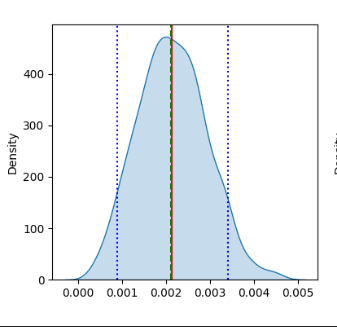
\includegraphics[width=\textwidth]{img/curvelambda.png}
		\caption{Paramètre $\lambda$}
		\label{fig:fig_simus_a}
	\end{subfigure}
	\hfill
	\begin{subfigure}{0.45\textwidth}
		\centering
		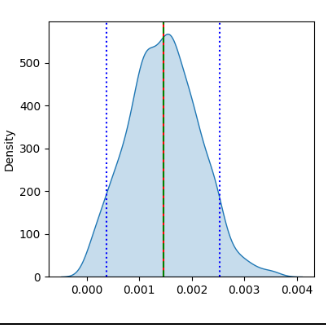
\includegraphics[width=\textwidth]{img/curvemu.png}
		\caption{$\mu$}
		\label{fig:fig_simus_b}
	\end{subfigure}
	\caption{\textbf{Relation entre les paramètres $\lambda$ (taux de copie) et $\mu$ (taux de perte) après inférence.}}
	\label{fig:fig_simus}
\end{figure}

La valeur \textit{a posteriori} du paramètre $\lambda$ qui représente, rappelons-le, la probabilité de copie d'un témoin, converge vers 0,002. Nous constatons d'ailleurs que la densité présente une concentration marquée autour de cette valeur centrale, tandis que l'intervalle d'incertitude demeure relativement restreint. Des observations similaires s'appliquent au paramètre $\mu$, représentant le taux de mort des témoins, estimé à 0,0015. Ces valeurs des paramètres $\mu$ et $\lambda$ constituent donc celles qui permettent de reproduire au mieux notre jeu de données empiriques, soit de restituer avec la plus grande fidélité possible la situation historique de nos manuscrits de textes patristiques. Il convient néanmoins de garder à l'esprit que cette inférence qui repose sur un processus de naissance-mort de type Poisson, se révèle en partie insatisfaisante. En effet, elle ne parvient pas à reproduire correctement le nombre total de textes ainsi que le nombre maximal de témoins par texte. Les estimations des paramètres $\mu$ et $\lambda$ demeurent donc très probables pour le jeu de données simulé actuel, qui ne reflète pas complètement notre réalité empirique.



\subsection{Résultats de l'inférence bayésienne sur nos données modélisées à l’aide d’un processus de naissance-mort de type Yule}

La dernière approche que nous avons explorée du projet \textit{LostMA} consiste à modéliser nos données à l’aide d’un processus de naissance-mort de type Yule. Cette orientation découle du constat précédent que la modélisation à l’aide d’un processus de naissance-mort simple, de type Poisson, s’est révélée inadéquate pour rendre compte de la distribution observée dans nos données. En effet, dans ce type de modèle, chaque manuscrit a une probabilité fixe et indépendante d’être copié ou de disparaître, ce qui génère une distribution exponentielle du nombre de témoins par œuvre. Or, une telle distribution se caractérise par une décroissance rapide : plus un texte possède de copies, plus la probabilité qu’il en ait encore davantage devient faible. Autrement dit, les textes très largement diffusées deviennent statistiquement improbables. Pourtant, l’analyse empirique des corpus de textes et de manuscrits médiévaux et patristiques montre clairement l’inverse. Pour un phénomène tel que la transmission textuelle, on a constaté que certains textes qui ont connu un large succès à un moment donné, laissent derrière eux un nombre de témoins bien plus élevé que d'autres. Dans notre corpus, par exemple, nous avons vu que des textes comme le corpus prudencien ou les \textit{Evangeliorum libri IV} de Juvencus présentent un nombre de témoins remarquablement élevé, que le modèle exponentiel ne peut expliquer.  Comme nous l'avons déjà souligné, cela s’est manifesté par l’incapacité de l’inférence à apprendre correctement le nombre maximal de témoins par texte et le nombre de textes lors de la modélisation par le processus de naissance-mort Poisson. L’intérêt du modèle de Yule réside donc dans sa capacité à mieux reproduire une loi à queue lourde de type parétienne, qui correspond mieux à la distribution observée dans nos données.

Lorsque Yule propose son modèle en 1924 dans l'article « A Mathematical Theory of Evolution »\footcite{yule1925}, il part d’une observation empirique faite en biologie : certaines catégories taxonomiques, comme les genres ou les familles, regroupent un nombre très inégal d'espèces. Par exemple, certains genres peuvent n’avoir qu’une ou deux espèces, tandis que d'autres en comptent des centaines. Cette distribution inégale semblait difficile à expliquer par le simple hasard ou par des caractéristiques biologiques particulières de chaque groupe. Yule cherche donc à formaliser mathématiquement ce phénomène, en introduisant un modèle de naissance fondé sur un processus de spéciation. Ce mécanisme repose sur l’idée que chaque espèce possède, à tout moment, une probabilité constante de donner naissance à une nouvelle espèce. Dans cette logique, les lignées qui connaissent davantage d’événements de spéciation au cours de leur histoire finiront, mécaniquement, par générer plus d’espèces. Autrement dit, même si toutes les espèces ont les mêmes chances de se diversifier, certaines lignées forment de très grands groupes simplement par effet cumulatif du hasard. Ce modèle prédit ainsi une loi de puissance dans la répartition d'espèces par genre.

Si l'on transpose cette logique à notre contexte de transmission textuelle, cela veut dire que contrairement à un modèle de naissance-mort type Poisson, chaque copie de texte n'a pas qu'une probabilité de générer une autre copie ou de s'éteindre. Elle peut donner lieu à une nouvelle espèce, c’est-à-dire à un nouveau texte : le modèle de Yule permet ainsi de générer de nouveaux \textit{stemmata}. La création d’un nouveau \textit{stemma} s’effectue selon deux modalités : soit par dérivation, ce qui peut être compris, comme le précise l’article « One Tree to Yule Them All? Reflexions on Intertextuality and Text Transmission »\footcite[p.1--2]{yule12tree}, comme une certaine forme d’intertextualité. La dérivation correspond à la production d’une nouvelle version d’un texte, que ce soit par une traduction, une mise en prose, une glose, etc. Le texte original et le texte dérivé entretiennent alors des relations d’intertextualité. Ce phénomène est bien attesté dans les traditions narratives médiévales et chevaleresques, telles que celles étudiées par le projet \textit{LostMA}. On peut notamment citer \textit{La Chanson de Roland}, qui connaît plusieurs versions dont notamment celles rimée et assonancée. Notre tradition patristique, en revanche, n’est pas marquée par de tels phénomènes de dérivation. Nous pouvons certes remarquer que certains textes de notre corpus s’inscrivent dans une logique d’intertextualité, mais c'est une forme différente de celle liée à la dérivation. Il ne s’agit plus simplement de transposer un texte en modifiant sa forme, sa langue ou son genre, mais plutôt de considérer l’influence qu’un texte a pu exercer sur un autre. Cette intertextualité, qu’elle soit explicite ou implicite, peut prendre des formes variées : emprunts, citations, mentions, références ou allusions. Ces procédés poursuivent souvent plusieurs objectifs, parfois complémentaires : approfondir ou prolonger une pensée théologique, s’inscrire dans la continuité et la perpétuation d'une tradition littéraire, ou tout simplement flatter l’oreille d’un public lettré. Nous citerons à nouveau cet exemple pour illustrer notre propos : l’œuvre de Prudence, largement reçue et reprise par des auteurs tels que Corippe, Sédule, Venance Fortunat, mais aussi, de manière plus étendue, dans la poésie carolingienne ou encore dans la liturgie mozarabe\footcite{receptionpaulinprudence}. Ce dernier type d’intertextualité ne sera donc pas retenu dans notre modélisation des processus de transmission textuelle : bien que les deux textes puissent entretenir des liens intertextuels, ils relèvent de traditions manuscrites distinctes et évoluent indépendamment l’un de l’autre. À l’inverse, dans le cas d’une intertextualité fondée sur la dérivation, les deux textes partagent une même tradition manuscrite, en ce sens que l’un constitue une forme de spéciation de l’autre, tous deux appartenant alors au même \textit{stemma}. La seconde modalité est celle de l’innovation : il s’agit de la naissance de nouveaux textes, produits indépendamment des arbres déjà existants. Elle correspond donc à l’apparition de textes originaux, non issus d’une tradition préexistante ce qui est très commun dans le phénomène de transmission textuelle.

Le modèle de Yule, à la différence du modèle de type naissance-mort de Poisson, repose ainsi sur quatre paramètres :

\begin{itemize}
	\item $\Lambda$ : probabilité de création d’arbres indépendants. 
	\item $\lambda$ : probabilité de reproduction.
	\item $\gamma$ : probabilité de spéciation.
	\item $\mu$ : probabilité d’extinction.
\end{itemize}

L’inférence à partir du modèle de Yule, bien que nous ayons établi qu’il était théoriquement mieux adapté à la nature de nos données, n’a pour l’instant donné aucun résultat satisfaisant. Nous avons mené vingt tentatives d’inférence en faisant varier à chaque fois le nombre d’échantillons et de simulations ainsi que la taille de la population initiale. Or, dans tous les cas, l’inférence échouait : la population simulée dépassait systématiquement le seuil maximal d’individus que nous avions fixé. Nous donnons une hypothèse sur ce qui conduit à cet échec : le modèle de Yule, en intégrant les paramètres de spéciation et d’innovation, tend à faire exploser notre population de témoins. En effet, le modèle de Yule a été conçu initialement pour des corpus d’œuvres médiévales produites entre le XIII\textsuperscript{e} et le XV\textsuperscript{e} siècle, dans lesquels de nouveaux textes apparaissent tout au long de la période. Or, notre cas s’en distingue profondément : bien que la transmission manuscrite de nos textes se prolonge jusqu’au XV\textsuperscript{e} siècle, aucun nouveau texte n’est créé après le V\textsuperscript{e} siècle. Durant l’Antiquité tardive, des textes sont effectivement produits, mais à partir du Moyen-Âge, ils ne font plus l’objet que d’une transmission. Le modèle ne permet pas de distinguer cette période de création textuelle d’une période de simple transmission. Ainsi, notre durée de période active 
est trop importante et laisse mécaniquement plus de temps, dans le cadre du modèle, à la spéciation et à l’innovation. Cela explique, selon nous, l’emballement de la population simulée, avec pour conséquence directe la création excessive d’arbres.


\subsection{Conclusion partielle}

Cette dernière étape de notre étude a consisté à appliquer, en nous appuyant sur les travaux récents du projet \textit{LostMA}, un modèle stochastique de type naissance-mort à notre corpus de textes patristiques, enrichi par une inférence bayésienne et des simulations multi-agents. Il s’agissait de tenter d’estimer les paramètres les plus probables expliquant la configuration actuelle du corpus. Avec le modèle de type Poisson, les résultats se sont révélés partiellement satisfaisants : certaines statistiques (nombre total de témoins, nombre de singletons, médiane de témoins par texte) sont bien reproduites. Toutefois, des écarts significatifs subsistent, en particulier sur le nombre de textes simulés ou les extrêmes de diffusion, ce qui souligne les limites de ce modèle. L’introduction du modèle de Yule permet d’affiner cette approche en intégrant une distribution plus réaliste, proche d'une loi à queue très lourde, mieux adaptée à la structure déséquilibrée des données. En pratique toutefois, ce modèle n’a pas donné de résultats exploitables : l’inférence échoue systématiquement, à cause d'une explosion de la population simulée. Cela suggère qu’une adaptation du modèle sera nécessaire à l’avenir pour mieux prendre en compte les spécificités historiques et dynamiques de notre corpus, en particulier la distinction entre une phase de création de textes concentrée dans l’Antiquité tardive et une phase de simple transmission et copie des manuscrits qui s’étend jusqu’au Moyen Âge. Pour ce faire, il faudrait combiner les deux modèles. Du III\textsuperscript{e} au V\textsuperscript{e} siècle, on aurait une première phase active de création de textes et de copie de manuscrits, à laquelle il conviendrait d’appliquer un modèle de Yule afin de rendre compte du phénomène de spéciation et de l’apparition de nouveaux textes. Du VI\textsuperscript{e} au XV\textsuperscript{e} siècle, on observerait une deuxième phase d’activité, cette fois modélisée par un processus de type Poisson, car durant cette période, seul le mécanisme de transmission est véritablement actif. Enfin, on conserverait une phase d’inactivité après le XVe siècle, durant laquelle le taux de copie chute drastiquement, laissant place principalement à un phénomène d’extinction et de conservation.

%Ces résultats rappellent que la survie ou la disparition des textes obéit à des dynamiques complexes, où hasard, contingence et choix culturels interfèrent

\chapter*{Conclusion}

Ce mémoire a permis d’explorer de manière inédite plusieurs aspects de la transmission textuelle des Pères de l’Église en péninsule Ibérique à travers des méthodes computationnelles.

La première étape de notre travail a consisté à caractériser le corpus lui-même. Il se distingue par sa diversité formelle et générique. Il contient à la fois des textes en prose et en vers, et couvre des genres variés : sermons, homélies, correspondances épistolaires, essais, chroniques historiques ou encore projets explicitement poétiques. De même, la taille des textes varie sensiblement : certains, comme les sermons ou les homélies, relèvent de la forme courte, tandis que d’autres, comme les épopées chrétiennes, sont des compositions longues et complexes.
Cette diversité interne a permis de mettre en évidence certaines dynamiques de transmission antagonistes. Les textes en prose ont globalement été plus abondamment conservés, mais ils ont souvent été transmis avec un nombre réduit de témoins. À l’inverse, la poésie, bien que moins représentée en nombre de textes, compte quelques grandes œuvres massivement diffusées. Ce déséquilibre du corpus se manifeste de manière particulièrement nette dans le cas de Prudence, dont les textes sont attestés dans près de 300 manuscrits sur un total d’environ 1159 manuscrits. Il s’agit là d’un biais de transmission humain et non aléatoire : la popularité d’un texte a favorisé sa copie, sa diffusion et, \textit{in fine}, sa conservation. 
Le corpus présente également une particularité notable liée à sa chronologie. En tant que production de l’Antiquité tardive, il a souvent été transmis dans le cadre de collections médiévales, rassemblées sous une unité qui peut être thématique ou générique. Certains textes doivent ainsi leur préservation à leur intégration dans des homéliaires, d’autres à leur inclusion dans des recueils canoniques. On observe donc un phénomène de conservation par collection, où le fait qu’un texte soit inséré dans une « anthologie » contribue à sa survie, parfois indépendamment de son auteur, de son authenticité ou même de son contenu initial. D’ailleurs, on remarque que cette intégration concerne majoritairement des textes en prose, ce qui pourrait en partie expliquer pourquoi la prose est surreprésentée parmi les textes conservés.
Ce déséquilibre dans la transmission nous a ainsi amené à constater que notre corpus suivait une loi à queue lourde, ce qui est typique des phénomènes culturels ou sociaux .

Ce mémoire a aussi été l’occasion d’aborder brièvement la question des \textit{stemmata codicum} et d’en observer certaines limites pour une analyse computationnelle : ils ne présentent pas tous le même niveau de précision (certains concernent les témoins, d’autres des familles de manuscrits), et dans certains cas, un même \textit{stemma} peut regrouper plusieurs textes d’un même auteur. Cette hétérogénéité rend leur traitement difficile à automatiser. Comment intégrer ces données dans un modèle computationnel cohérent, sans aplatir ou forcer leur complexité ? C’est une question restée ouverte. Sur les propriétés proprement stemmatiques de notre tradition, nous n’irons pas plus loin ici : le nombre de \textit{stemmata} disponibles est encore trop limité pour permettre une véritable conclusion.

Une difficulté méthodologique majeure rencontrée tout au long du mémoire a été le niveau de granularité que nous accordions au témoin, qui est différent du manuscrit. Cette question a constitué un véritable défi pour la modélisation : comment déterminer le niveau de précision pertinent pour une analyse computationnelle ? Quels sont les critères pour que des textes forment un corpus, et que faut-il traiter comme des unités indépendantes ? Ce problème était particulièrement délicat dans le cas de notre corpus, où les textes d’un même auteur sont souvent portés par une cohérence doctrinale et thématique et relèvent ainsi d’une même tradition manuscrite. Il a donc fallu trouver le bon équilibre entre une simplification excessive et une segmentation trop fine.

Enfin, les modélisations de la transmission textuelle que nous avons mises en œuvre ont apporté des résultats intéressants. La méthode des espèces non vues, développée par M. Kestemont et son équipe nous a permis de dégager quelques premières valeurs indicatives : environ une centaine de textes patristiques, au minimum, auraient vu le jour dans la péninsule Ibérique. Parmi ceux-ci, seuls environ 10\,\% des témoins manuscrits sont aujourd’hui identifiés, ce qui témoigne d’une perte significative au sein de la tradition manuscrite. Cette hypothèse est renforcée par les indices de diversité, notamment l’équitabilité, qui indiquent que notre corpus est loin d’être équilibré et donc particulièrement vulnérable à la disparition de textes.


Le second type de modélisation que nous avons employé pour appréhender la transmission textuelle est de nature stochastique. Ce type de modèle permet non seulement d’évaluer les taux de perte et de survie des textes ou des manuscrits, mais aussi d’explorer des dynamiques de population au fil du temps. Son application à notre corpus patristique ne s’est pas soldée par des résultats véritablement concluants.
Le premier modèle testé, basé sur une loi de Poisson, ne semblait pas pleinement adapté à nos données, qui suivent une loi à queue lourde. Ce constat avait d’ailleurs déjà été formulé par l’équipe du projet \textit{LostMA}, sur un type de tradition tout à fait différent, les récits chevaleresques. À l’inverse, le modèle de Yule semble offrir une meilleure alternative, plus apte à rendre compte des phénomènes de création et de diversification des textes. Nous avons tenté de l’appliquer mais sans résultats significatifs. Là encore, c’est probablement l’inadéquation entre le modèle et les spécificités de notre corpus qui explique cet échec.

Notre corpus se distingue en effet par la coexistence de plusieurs phases : une période de création textuelle suivie d’une période de simple transmission. Or, cette distinction temporelle entre genèse de nouveaux textes et simple reproduction  n’est pas prise en compte par les modèles actuels. Intégrer cette différence constituerait une amélioration nette du modèle pour notre corpus, et c’est d’ailleurs l’un des objectifs majeurs à poursuivre dans la suite de ce travail.

Enfin nous avons souligné à plusieurs reprises dans ce travail que notre corpus repose sur une petite population, ce qui peut parfois limiter la robustesse statistique de certaines analyses. Comme précisé précédemment, le travail de collecte des manuscrits et des textes a été exhaustif pour la période et la zone géographique considérées. Toutefois, pour obtenir des résultats plus probants et plus généralisables, il serait pertinent d’étendre le corpus de textes patristiques à d’autres aires culturelles, comme l’Africanie ou la Gaule. Ce serait un chantier ambitieux et de longue haleine, mais qui ouvrirait des perspectives passionnantes pour la modélisation de la transmission textuelle patristiques à plus grande échelle.

En somme, ce travail a permis de croiser les approches philologiques et computationnelles les plus actuelles pour interroger la transmission textuelle d'une tradition inédite, les textes patristiques de la péninsule Ibérique. Les résultats obtenus ouvrent la voie à d'autres modélisations, et à des comparaisons avec d'autres corpus.




	


%\clearpage




\appendix
\part*{Annexes}
\chapter{Arbres stemmatiques}

\section{Arbres stemmatiques représentant un biais pour les analyses computationnelles}
\label{stemmabifid}
\begin{figure}[p]  
	\centering
	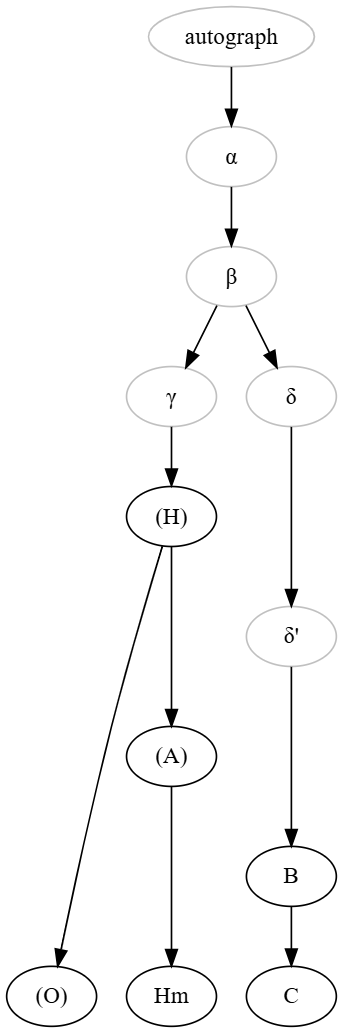
\includegraphics[width=0.4\linewidth]{img/stemmaIdace.png}
	\caption{\textit{Stemma codicum} des \textit{Chroniques} d'Hydace.}
	\label{fig:stemma1}
\end{figure}

\begin{figure}[p]  
	\centering
	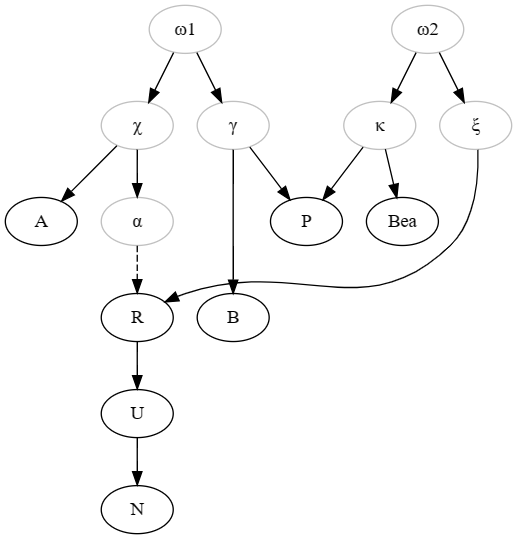
\includegraphics[width=0.8\linewidth]{img/stemmagregorius.png}
	\caption{\textit{Stemma codicum} du \textit{Tractatus V de epithalamio} de Grégoire d'Elvire.}
	\label{fig:stemma1}
\end{figure}


\begin{figure}[p]  
	\centering
	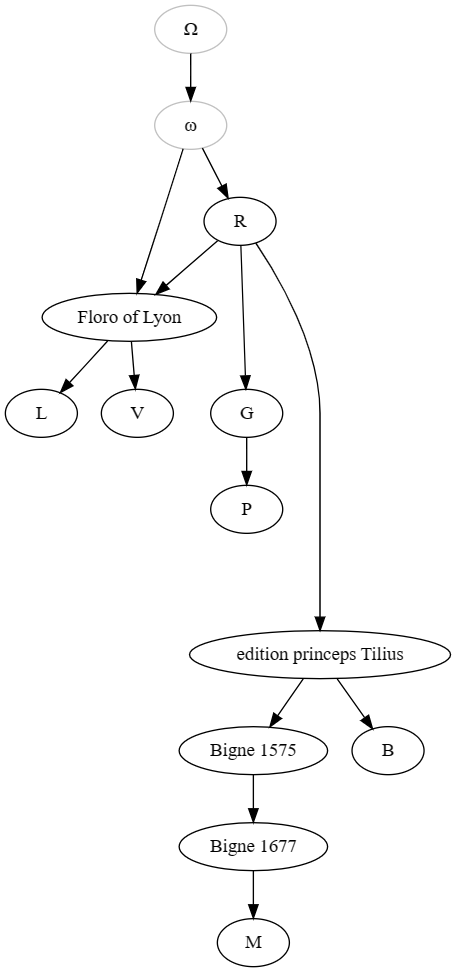
\includegraphics[width=0.7\linewidth]{img/stemmapacien.png}
	\caption{\textit{Stemma codicum} des textes de Pacien de Barcelone.}
	\label{fig:stemma1}
\end{figure}

\chapter{Les estimateurs de richesse}

\section{Critères d'estimation des différents estimateurs de richesse}


\begin{table}[h!]
	\centering
	\renewcommand{\arraystretch}{1.5} % Augmente l'espacement des lignes
	\resizebox{\textwidth}{!}{
		\begin{tabular}{|l|l|l|}
			\hline
			\textbf{Estimateur} & \textbf{Principe} & \textbf{Ajustement supplémentaire} \\
			\hline
			Chao1 & Estime la richesse en se basant sur les singletons et doubletons. & Aucun ajustement supplémentaire. \\
			\hline
			iChao1 & Ajuste Chao1 en ajoutant des comptages pour les tripletons et quadrupletons. & Prise en compte de  $f_3$ et  $f_4$. \\
			\hline
			ACE & Estime la richesse en fonction des fréquences d'espèces rares et leur abondance. & Ajustement basé sur un seuil \textit{k}. \\
			\hline
			Egghe \& Proot & Ajuste la richesse en utilisant les fréquences des espèces observées une ou deux fois. & Facteur de correction basé sur un paramètre $\alpha$. \\
			\hline
			Jackknife & Estime la richesse en rééchantillonnant les données en excluant successivement des observations. & Réévaluation des sous-échantillons. \\
			\hline
		\end{tabular}
	}
	\caption{Résumé des différents estimateurs de richesse.}
	\label{tab:estimateurs}
\end{table}

\chapter{Annexes numériques}

Pour accéder au code et aux données associés à ce mémoire, veuillez consulter le dépôt GitHub suivant :\\
\url{https://github.com/Emiliegd14/IberianChurchFather_tradition}



\backmatter

\listoffigures
\tableofcontents

\end{document}
